\documentclass[a4paper,11pt, openany]{book}
\usepackage[utf8]{inputenc}
\usepackage[T1]{fontenc}
\usepackage[english, french]{babel}
\usepackage[paper=a4paper]{geometry}
\usepackage{layout}
\usepackage{float}
\usepackage{eso-pic, graphicx, transparent}
\usepackage{wrapfig}
% \usepackage{times}
% \usepackage{float}
\usepackage{lmodern}
% \usepackage{amsmath}
% \usepackage{amssymb}
% \usepackage{hyperref}
% \usepackage{caption}
% \usepackage{placeins}
\usepackage{setspace}
\usepackage{indentfirst}
\usepackage{fancyhdr}
\usepackage{lipsum}
\usepackage{array}
\usepackage{titlesec}

\usepackage{listings} %insérer code

\usepackage{subfigure}
\usepackage{tikz}

\usepackage{appendix}


% FORMULES
\usepackage{amsmath}
\usepackage{amssymb}
\usepackage{mathrsfs}
\usepackage{array}
% \usepackage{subcaption}
% \usepackage{titlesec}
% \usepackage{enumitem}


\usepackage[automake]{glossaries-extra}


\setabbreviationstyle[acronym]{long-short}
\makeglossaries


% \newglossaryentry{activations_musculaires}{name=activations musculaires, description={ - }}


\newglossaryentry{biorbdoptim}{name=BiorbdOptim, description={ --- }}
\newglossaryentry{biorbdviz}{name=BiorbdViz, description={ --- }}
\newglossaryentry{biorbd}{name=Biorbd, description={ --- }}
\newglossaryentry{travis}{name=Travis CI, description={ --- }}
\newglossaryentry{black}{name=Black, description={ --- }}
\newglossaryentry{eigen}{name=Eigen, description={ --- }}
\newglossaryentry{moco}{name=MoCo, description={ --- }}
\newglossaryentry{anaconda}{name=Anaconda, description={ --- }}
\newglossaryentry{pycharm}{name=PyCharm, description={ --- }}
\newglossaryentry{qt}{name=Qt, description={ --- }}
\newglossaryentry{linux}{name=Linux, description={ --- }}
\newglossaryentry{numpy}{name=NumPy, description={ --- }}
\newglossaryentry{scipy}{name=SciPy, description={ --- }}
\newglossaryentry{matplotlib}{name=Matplotlib, description={ --- }}
\newglossaryentry{pickle}{name=Pickle, description={ --- }}
\newglossaryentry{casadi}{name=CasADi, description={ --- }}
\newglossaryentry{acados}{name=ACADOS, description={ --- }}
\newglossaryentry{ipopt}{name=Ipopt, description={ --- }}
\newglossaryentry{slack}{name=Slack, description={: plate-forme de communication collaborative ---}}
\newglossaryentry{zoom}{name=Zoom, description={: service de téléconférence ---}}
\newglossaryentry{teams}{name=Teams, description={: application de communication collaborative ---}}
\newglossaryentry{github}{name=GitHub, description={: service de gestion de développement de logiciels individuel ou collectif ---}}
\newglossaryentry{gitkraken}{name=GitKraken, description={: interface graphique pour logiciels de gestion de développement de logiciels ---}}
\newglossaryentry{pomodoro}{name=pomodoro, description={: technique de gestion du temps avec alternance de temps de travail (25 minutes) et de pauses (5 minutes) ---}}

\newacronym{mhe}{MHE}{Moving horizon estimation ---}
\newacronym{ieee}{IEEE}{Industrial Electronics Society ---}

\hfuzz=20pt
\vfuzz=20pt
\hbadness=2000
\vbadness=\maxdimen


\hypersetup{colorlinks=True, linkcolor=black, citecolor=black,  filecolor=black, urlcolor=black}

\lstset{language=Python, linewidth=0.8\textwidth, backgroundcolor=\color{yellow!20}, frame=single, numbers=left, xleftmargin=0.2\textwidth, showspaces=false}

\setlength{\DTbaselineskip}{20pt}
\DTsetlength{1em}{1.5em}{0.5em}{1.2pt}{5pt} %{offset}{width}{sep}{rule-width}{dot-size}

\pdfminorversion=7

\setlength{\hoffset}{-18pt}        
\setlength{\oddsidemargin}{0pt} % Marge gauche sur pages impaires
\setlength{\evensidemargin}{9pt} % Marge gauche sur pages paires
\setlength{\marginparwidth}{54pt} % Largeur de note dans la marge
\setlength{\textwidth}{481pt} % Largeur de la zone de texte (17cm)
\setlength{\voffset}{-60pt} % Bon pour DOS
\setlength{\marginparsep}{7pt} % Séparation de la marge
\setlength{\topmargin}{0pt} % Pas de marge en haut
\setlength{\headheight}{13pt} % Haut de page
\setlength{\headsep}{15pt} % Entre le haut de page et le texte
\setlength{\footskip}{27pt} % Bas de page + séparation
\setlength{\textheight}{708pt} % Hauteur de la zone de texte (25cm)


\pagestyle{fancy}
\setlength{\headheight}{51pt}

% Head page
\fancyhead[L]{
\includegraphics[height=1.2cm]{images/logo_emse_long.jpg}}
\fancyhead[C]{\leftmark}
\fancyhead[R]{
\includegraphics[height=1.4cm]{images/logo_s2mlab_long.jpg}}
\renewcommand{\headrulewidth}{0.4pt}

% Foot page
\fancyfoot[C] {\thepage}
\renewcommand{\footrulewidth}{0.4pt}




\newcommand\tab[1][1cm]{\hspace*{0.5cm}}

\title{Rapport de stage}
\author{Théophile \textsc{GOUSSELOT}}




\begin{document}
\titleformat{\chapter}[display]{\normalfont\bfseries}{}{0pt}{\Huge\thechapter.\ }

\onehalfspacing %interligne de 1.5 (package setspace)
% \setlength{\parskip}{0.5cm}


\renewcommand{\contentsname}{Sommaire}
\frontmatter
\newcommand\imagepagedegarde{ \put(90,250){ \parbox[b][\paperheight]{0.7\paperwidth}{ \vfill \centering 

\includegraphics[width=4cm, height=4cm]{images/logo_s2mlab.jpg}
\hfill
\includegraphics[width=4cm, height=4cm]{images/logo_emse.png}
\vfill }}}

\newcommand\imagedefond{ \put(11,-182){ \parbox[b][\paperheight]{\paperwidth}{ \vfill \centering \transparent{0.7}\includegraphics[width=18cm, keepaspectratio]{images/logo_emse_fond2.png}\vfill }}}


\begin{titlepage}
\AddToShipoutPicture*{\imagedefond}
\AddToShipoutPicture*{\imagepagedegarde}

    \begin{center}
    
    \phantom{}
    
    \vspace{5.5cm}
    
    \LARGE{Rapport de fin de stage internationnal}
    
    \rule{\linewidth}{0.5mm}\\
    {\huge \bfseries Optimisation du mouvement du violoniste afin de minimiser la fatigue musculaire \\}
    \rule[0.25cm]{\linewidth}{0.5mm}\\[2.7cm]
    \end{center}
    
        
    \begin{flushright}
    \begin{minipage}[c]{10.8cm}
        {\itshape \bfseries \'Etudiant :}\\
        \tab Théophile \textsc{Gousselot EI18}\par
        \vspace{0.3cm}
        {\itshape \bfseries Tuteur pédagogique :}\\
        \tab David \textsc{Moreau}\par
        \vspace{0.3cm}
        {\itshape \bfseries  Tuteur laboratoire :}\\
        \tab Benjamin \textsc{Michaud}\par
        \vspace{0.3cm}
        {\itshape \bfseries  Directeur du laboratoire :}\\
        \tab Mickaël \textsc{Begon}\par
    \end{minipage}
    \end{flushright}
    

    \begin{center}
    \begin{minipage}[c]{8cm}
    \vspace{4cm}
%     \rule{\linewidth}{0.2mm}\\
%     {\large Effectué du 18 Mars 2020 au 04 Août 2020}
%     \rule[0.25cm]{\linewidth}{0.2mm}
    
    \begin{tabular}{c}
    \hline
    Effectué du 18 Mars 2020 au 04 Août 2020 \\
    \hline
    En télétravail depuis Montréal\\
    \hline
    \end{tabular}
    

    \end{minipage}
    \end{center}
\end{titlepage} 

\newpage
\addcontentsline{toc}{part}{Résumé}
\textbf{\huge Résumé}
\vspace{0.5cm}\\\tab
Le présent rapport s'intègre au sein d'une thèse portant sur l’optimisation du mouvement du violoniste afin de minimiser la fatigue musculaire. Ma contribution à ce projet fut parallèlement partagée entre le développement d'un outil générique de contrôle optimal : \emph{BiorbdOptim}, et l'optimisation du mouvement du violoniste grâce à cet outil.\emph{BiorbdOptim} est une interface entre un utilisateur et un solveur de problèmes de contrôle optimal. Cet outil est développé par et dans une première finalité, pour les chercheurs du laboratoire \emph{s2mlab}. L'utilisation de \emph{BiorbdOptim} et d'un modèle, issue de la librairie \emph{BIORBD}, des membres supérieurs humains portant un violon et son archet, m'a permis d'écrire un problème de contrôle optimal. Ce problème s'est progressivement raffiné, en intégrant successivement : le mouvement de tiré-poussé via des couples articulaires, le maintient du contact entre l'archet et la corde, le respect du parallélisme entre l'archet et le chevalet, le maintient du même angle pour l'archet, une force de contact entre l'archet et le violon, les muscles aux alentours du bras, une modélisation de fatigue musculaire, plusieurs mouvement successifs de tiré-poussé. %todo à compléter
La finalité de cette modélisation est de parvenir à déterminer le plus fidèlement possible, et par du contrôle optimal le mouvement minimisant la fatigue musculaire dans le but d’aider à l’enseignement du violon.

\vspace{1.5cm}
\textbf{\huge Abstract}
\vspace{0.5cm}\\\tab
This report is part of a thesis on the optimization of the violinist's movement in order to minimize muscular fatigue. My contribution was shared between the development of a generic optimal control tool: \emph{BiorbdOptim}, and the optimization of the violinist's movement thanks to this tool. \emph{BiorbdOptim} is an interface between a user and a solver of optimal control problems. Further, it is developed by and also for the researchers of the s2mlab laboratory. The use of BiorbdOptim and a model of human upper limbs carrying a violin and its bow, from the \emph{BIORBD} library, allowed me to write an optimal control problem. This problem has been progressively enhanced, successively integrating these concepts : the back and forth movement via articular couples, maintaining contact between the bow and the string, respecting parallelism between the bow and the bridge, maintaining the same angle for the bow, a contact force between the bow and the violin, the muscles around the arm, a model of muscular fatigue, several successive pull-push movements. %todo to be completed
The purpose of this modeling is to determine as accurately as possible, and through optimal control, the movement that minimizes muscle fatigue in order to assist in the teaching of the violin.






\newpage
\addcontentsline{toc}{part}{Remerciements}
\textbf{\Huge Remerciements}
\vspace{0.5cm}\\\tab

Mickaël BEGON
Benjamin MICHAUD
David MOREAU

Paul WEGIEL

Ariane DANG
Kilpéric NOUVELLET
Quitterie BOISS\'E
Amedeo CEGLIA
Bailly FRANCOIS
Léa SANCHEZ

Eve CHARBONNEAU
Najoua ASSILA

Clara ZIANE

Fabien DEL MASO
Béatrice MOYEN-SYLVESTRE
Anne Laure M\'ENARD
+ tout le laboratoire


Klara NOVOTNA
Frédérique Alexandre MICHAUD : Les évènements culturels rythmant les été de Montréal -> FAM


Bruno MONSARRAT
Les familles SOLAR

Sylvie et Philippe GOUSSELOT

Camille WILHELM


\newpage
\begin{flushright}
\phantom{}
\vspace{2cm}
\textit{\'A mes amis musiciens, et à ceux qui aiment la musique...}\par
\vspace{1.5cm}
\end{flushright}
\begin{figure}[h]
\begin{center}
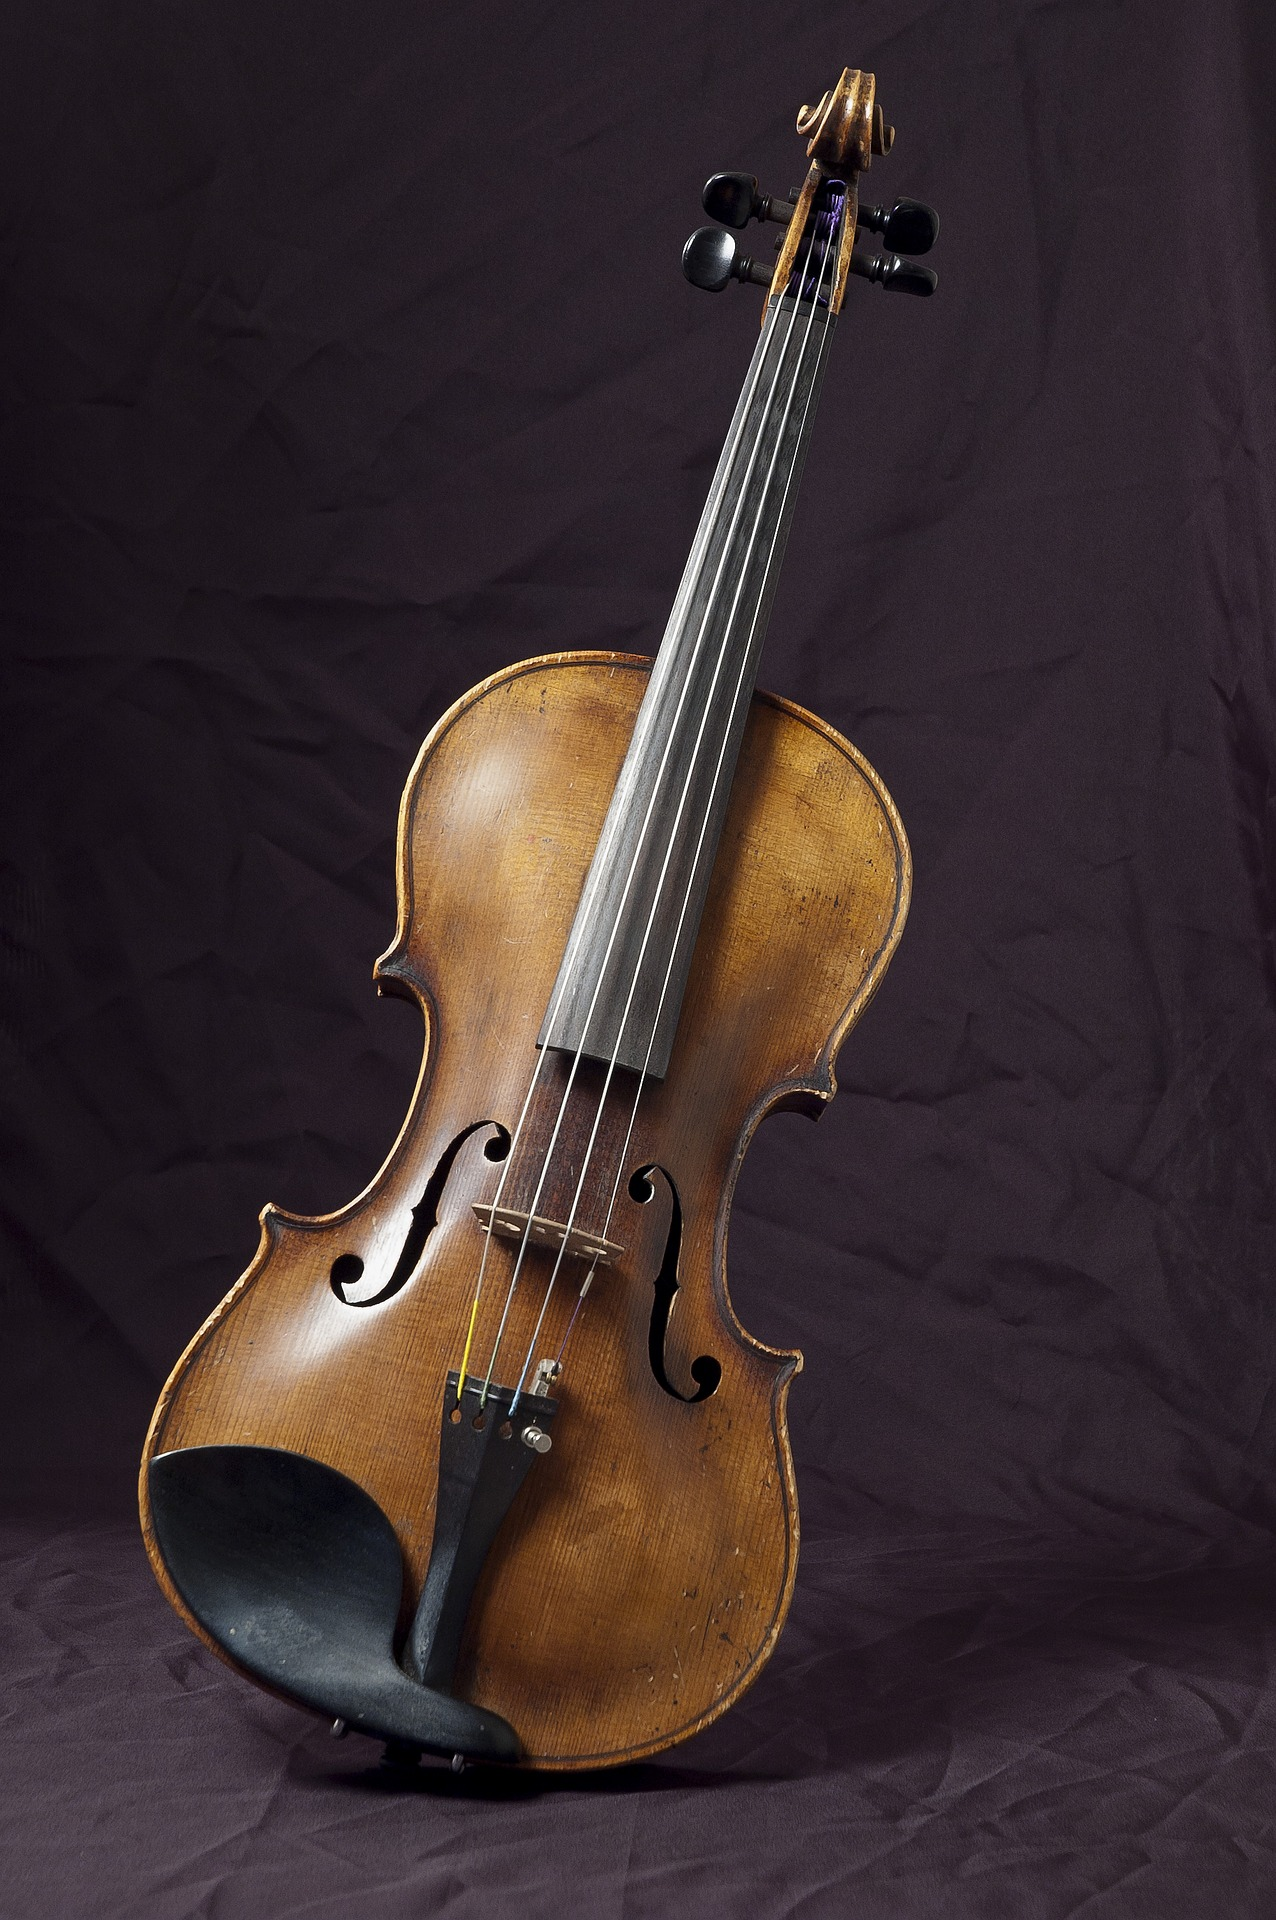
\includegraphics[width=10cm]{images/violin_cover.jpg}
\caption{Un violon muni d'une mentonnière .}
\end{center}
\end{figure}
\par La mentonnière, utilisée pour la première fois au début du XIX\textsuperscript{ème} siècle, est une des premières adaptation du violon au corps du musicien, elle sépare la sueur du violoniste du violon afin de ne pas altérer le vernis à sa surface.

\^A l'image de la mentonnière, mon travail est de perfectionner le ``couple'' du musicien et de son violon.

\renewcommand{\contentsname}{Table des matières}
\setcounter{tocdepth}{6}
\begin{spacing}{0.9}
\tableofcontents
\end{spacing}


\renewcommand{\glossaryname}{Glossaire}
\printglossaries

\mainmatter
\part{Introduction}
    \chapter{Stage international}

Mon cursus à l'\'Ecole des Mines de Saint-Étienne me permet au deuxième semestre de deuxième année de réaliser un \emph{projet industriel} sur le campus ou un \emph{stage international}.
J'ai souhaité partir à l'étranger, l'expérience associée me semblant davantage complète et engageante. La dimension professionnelle du stage, mettant en jeu des interactions sociales différentes de celles rencontrées au sein d'associations et de groupes de projets étudiants en est la première raison. Mon choix s'est porté sur le Canada et la province du Québec. Principalement motivé par le laboratoire de simulation et modélisation du mouvement : \emph{s2m}, la culture québecoise et les splendides paysages ne m'ont que confortés dans ce choix.

Mme Camille \textsc{Wilhelm}, étudiante de la promotion précédente ayant réalisé un stage international au laboratoire s2m m'en a fait une présentation globale : activités de recherches, état d'esprit, encadrement et méthodes de travail. J'ai ensuite échanger avec M. Benjamin \textsc{Michaud}, ancien tuteur de Mme  Camille \textsc{Wilhelm}. La discussion a porté sur ses activités de recherches, ses besoins et mes compétences.
Cette série d'échange, entre autre, m'a permis de prendre conscience de l'intérêt de s'essayer à un travail de recherche et non industriel, dans l'optique d'appréhender fidèlement ces deux mondes.


    \chapter[Laboratoire s2m]{Laboratoire simulation et modélisation du mouvement}
        \section{Histoire}
        
En 2008, M. Mickaël \textsc{Begon} fonde le laboratoire de Simulation et Modélisation du Mouvement dont l’objectif est la recherche en biomécanique et la formation de personnel hautement qualifié en kinésiologie. D'abord installé dans les locaux du Centre de réadaptation Marie-Enfant à Montréal, le laboratoire migre à Laval en 2011, lors de la fondation du
nouveau campus de l’université de Montréal.


        \section{Domaine d'expertise}
        
Le laboratoire s2m est porté vers le développement de nouvelles connaissances sur la motricité humaine à
partir de mesures et de modèles de simulation pour des applications en réadaptation, prévention des
blessures et amélioration de la performance sportive et artistique. On peut citer des projets phares comme l'optimisation dynamique d'acrobaties, l'optimisation du geste violonistique et pianistique, ou encore la conception d’orthèses plantaires personnalisées. Les projets se rapportent tous à une thématique musicale, sportive ou ergonomique.
Le laboratoire S2M fonctionne majoritairement grâce aux subventions des organismes du
Québec et du Canada comme la fondation Canadienne pour l’innovation ou l’Institut de recherche en
Santé et Sécurité au travail. Il est aussi en relation avec des partenaires industriels. % toujours vrai ?


Le laboratoire bénéficie d’équipement de pointe pour les mesures biomécaniques : 
\begin{itemize}
\setlength\itemsep{-0.5em}
\item Un ergomètre isocinétique.
\item Un système optoélectronique de 18 caméras.
\item Un système EMG : Électromyographie (intramusculaire et de surface).
\item Des plateformes de force sur une piste de marche.
\item Un tapis instrumenté pour la marche.
\item Un piano acoustique.  
\end{itemize}
\newpage

    
        \section{Effectif}      
Supervisé par M. Mickaël \textsc{Begon} et M. Fabien \textsc{Del Maso}, le laboratoire de recherche universitaire s2mlab peut s'apparenter à un outil pédagogique de formation étudiante. L'effectif de recherche regroupe en moyenne 25 chercheurs. Il se renouvelle très régulièrement, allant du stagiaire de quelques mois à la thèse ou au doctorat de plusieurs années, à titre d'exemple, on peut dénombrer 6 arrivants lors de mon stage. L'objectif de ce renouvellement est de proposer à un maximum d'étudiants de vivre une expérience scientifique afin d’insuffler un goût pour la recherche, amenant certains à faire suite à leur stage avec une thèse ou un doctorat.
\begin{figure}[h]
\begin{center}
\begin{tikzpicture}[
    every node/.style = {shape=rectangle, rounded corners, draw, align=center, top color=white, bottom},
    level 1/.style={sibling distance=60mm},
    level 2/.style={sibling distance=30mm},
    level 3/.style={sibling distance=25mm}]]
    \node {S2mlab\\\footnotesize{(25 pers)}}
        child { node {Permanents}
            child { node {Assistants de\\recherche\\\footnotesize{(5)}} }
            child { node {Coordinateurs\\\footnotesize{(5)}} } }
        child { node {Temporaires}
            child { node {\'Etudiants}
                child { node {Postdoctoral\\\footnotesize{(5)}} }
                child { node {Thèse\\\footnotesize{(5)}} }
                child { node {Maitrise\\\footnotesize{(5)}} } } };
\end{tikzpicture}
\caption{Organigramme du laboratoire}
\end{center}
\end{figure}
\label{equipe_control_optimal}
Le laboratoire est découpé en plusieurs thématiques, en tant que stagiaire de Benjamin \textsc{Michaud}, j'ai rejoint l'équipe de \emph{optimal control}, \emph{commande optimale} en français. Composé d'une dizaine de chercheurs, l'équipe se réunit tous les mardi matin lors d'un tour de table où chacun expose ses avancées et ses problèmes. L'aspiration de cette réunion est double, débloquer rapidement les chercheurs qui sont en difficultés et s'assurer d'une collaboration efficace : jouir de l'expérience des autres chercheurs pour ne pas essayer de réinventer l'eau chaude. M. Mickaël \textsc{Begon}, professeur agrégé, participe à cette rencontre et apporte, entre autre, une vision biomécanique et un sens de l'efficacité.



        \section{Recherche scientifique}
        
Il est important de différencier la recherche scientifique de la recherche industrielle. Si la première se veut collaborative et nécessite le concours de plusieurs laboratoire, la deuxième est par nature concurrentielle afin de commercialiser en premier des technologies et de déposer des brevets.

%revenir sur la collaboration avec l'idée de se comparer articles BoirbdOptim (MOCO)

Un chercheur scientifique se doit donc de publier des articles afin de partager ses recherches à ses homologues. A travers ses articles, et les citations de ses articles, le chercheur peut appuyer ses demandes de financement. La recherche, n'engendrant pas de profit direct, nécessite de faire appel à des acteurs extérieurs. La collectivité assume en grande partie ce rôle en finançant les universités, qui finance ensuite le laboratoire s2mlab. %à vérifier !

%open source ??


    \chapter{Contexte}
        \section{Covid-19}
        
        
Lors de mon arrivé le 15/03/20, l'université de Montréal a fermé ses portes à la totalité de ses étudiants, professeurs et chercheurs. Les locaux du laboratoire s2m ont ainsi été fermés, privant les chercheurs de matériel expérimental et de certaines ressources informatiques.

        \section{Télétravail}

L'obligation de télétravail pour l’ensemble des chercheurs du laboratoire a nécessité la mise en place de plusieurs outils informatiques :

\begin{description}
\setlength\itemsep{-0.5em}
\item[Messagerie :] \emph{\gls{slack}} puis \emph{\gls{teams}}.
\item[Visioconférence :] \emph{\gls{zoom}}, comprenant une fonctionnalité de \emph{remote control} : prise de contrôle à distance de l'ordinateur.
\end{description}

En complément de ceux existants :

\begin{description}
\setlength\itemsep{-0.5em}
\item[Gestion de développement de logiciels :] \emph{\gls{github}} couplé avec \emph{\gls{gitkraken}}.
\item[Répartition de taches :] \emph{trello}.
\item[Partage de fichiers :] \emph{serveurs du laboratoire}.
\end{description}

En écartant \emph{trello} dont l'utilisation est rendue caduc par le système d'\emph{issue} proposé par \emph{github}, on peut considérer que 3 logiciels de communication permettent de répondre aux besoins émanants de collaboration.

\begin{table}[h]
\begin{center}
\begin{tabular}{|c|c|c|c|c|}
\hline
Mode & Temps & Type & \'Echéance & Logiciel\\
\hline
oral & long ($\simeq$ heure) & réflexions stratégiques/développement & long terme & \emph{zoom} \\
\hline
écrit & court ($\simeq$ min) & aide rapide, mémorisation par écrit  & court terme & \emph{microsoft teams} \\
\hline
écrit  &  instantané & fichiers de programmation (\textbf{code}) & court terme & \emph{github}, \emph{gitkraken} \\
\hline
écrit  &  court ($\simeq$ min) & liste d'idées (\textbf{issue}) & long terme & \emph{github}, \emph{gitkraken} \\
\hline
\end{tabular}
\end{center}
\end{table}

S'il est pertinent de remarquer qu'un échange oral permet un débat profond et efficace autour d'une stratégie de développement, on peut regretter l'éphémérité de l'information. Il est possible d'y palier en inscrivant l'information essentiel sur teams, sur les issues de github ou au sein des lignes de codes.

La répartition des échanges est simple, néanmoins, elle implique, à chaque instant, de réfléchir au moyen de communication le plus adapté.

Avec du recul, il est aisé de détecter un choix de communication inadapté, par exemple une discussion sur teams avec un nombre de messages important, laisse présager qu'une vidéoconférence aurait été davantage efficace. En revanche, une vidéoconférence sans prise de note, c'est à dire n'aboutissant pas à une issue, un message ou un commentaire dans le code, laisse présager une perte d'information.

Enfin, il faut garder à l'esprit qu'un outil de collaboration est là pour économiser du temps et préserver l'information utile, ce qui revient à économiser du temps. L'objectif étant de se concentrer davantage sur la recherche. Il faut ainsi toujours veiller à rester vigilant et lucide face à l'utilisation faite des outils de communications.


        \section{Construction d'équipe}
        
Le confinement étant de vigueur, les régulières activités de groupe du laboratoire ont été suspendues. Malgré cela, certaines activités ont pu se réinventer via logiciel de vidéoconférence :
\begin{itemize}
\setlength\itemsep{-0.5em}
\item Séance de sport.
\item Séance de yoga.
\item Escape-game en ligne.
\end{itemize}

Au fur et à mesure de l'assouplissement du confinement, des activités extérieures de groupe ont pu voir le jour, dans le respect des distances et des gestes barrières :
\begin{itemize}
\setlength\itemsep{-0.5em}
\item Séances de travail collectives en appliquant la technique \emph{\gls{pomodoro}} dans des parcs.
\item Randonnées et séances sportives.
\end{itemize}

La finalité de ces temps partagés avec des collègues chercheurs, est de casser la monotonie de télétravail depuis la maison. En télétravail, il est particulièrement complexe de dissocier les temps de travail des temps personnels. D'autant plus dans un cadre de recherche où l'avancement, et ainsi l'entrain varient. Il en résulte que mon temps de travail hebdomadaire est en moyenne supérieur à 35 heures par semaine, avec un temps de travail quotidien oscillant entre 6h et 9h.

Il s'est avéré que le simple fait de travail en visioconférence avec ses collègues, sans forcement discuter, permet au travers du bruit de fond et de leur présence de reconstituer un contexte de travail.

\part{BiorbdOptim}
    \chapter[Outils de modélisation]{Outils de modélisation numérique du mouvement}
    
    
Avant de rentrer dans le vif du sujet, il est nécessaire de définir et décrire quelques notions et logiciels sans quoi on ne peut comprendre l'intérêt ou le fonctionnement de \emph{\gls{biorbdoptim}}.

Le système d'exploitation \emph{\gls{linux}} a été le premier outil utilisé par la quasi-totalité des contributeurs à \gls{biorbdoptim}, il est intéressant de noter que la couche de compatibilité \emph{Windows Subsystem for Linux} a permis à quelques utilisateurs de travailler sur \gls{biorbdoptim} depuis le système d'exploitation \emph{Windows}. Afin de pouvoir simplifier la gestion des paquets et faciliter le déploiement du logiciel, la distribution libre et open source \gls{anaconda} a été grandement utilisée.

Enfin, la programmation en tant que telle, a été conduite grâce grâce aux environnements de développement \gls{pycharm} pour le langage python, et \gls{qt} pour le langage c++. ces deux environnements sont complets, ils proposent entre autre, un débogueur graphique, des outils de publication de code sur github ainsi que des licences étudiantes gratuites.
\label{pycharm}

        \section{Commande optimal}
        
%expliquer pourquoi on parle de commande optimal
\label{commande_optimale}
La commande optimale est une méthode utilisée dans le cas d’un problème de dynamique
régit par des équations différentielles. L’objectif est d’emmener le système d’un état initial jusqu’à un état final tout en maximiser ou minimiser des indices de performances nommées ``fonctions-objectifs'' et en respectant des contraintes.

L'utilisation de commande optimal est particulièrement approprié lorsque les mouvements d'un système sont dynamiques. A titre d'exemple, on l'utilise en biomécanique pour modéliser les mouvements du corps humain. La notion dynamique, réside ici dans l'impossibilité pour le système nerveux à contrôler la position finale d'un membre, son contrôle se limite à émettre un signal au muscle par le système nerveux. Le mouvement du membre est alors régit par des contraintes tels que le fonctionnement du muscle ou la gravité. 

Le principe consiste à agir sur les commandes (variables d’entrées) qui à partir des équations du système donnent les états différentiels du système dynamique. On vérifie ensuite si les contraintes sont respectées et si la valeur de la fonction objectif est plus petite qu’une limite pré-établie. Si c’est le cas, la valeur constitue la solution optimale, sinon on modifie les commandes selon un algorithme de gradient pour recommencer le processus.

Il est possible de schématiser le fonctionnement de la commande optimale comme suit :

\begin{figure}[H]
\begin{center}
\includegraphics[width=4cm]{images/control_optimal.png}
\caption{Principe de fonctionnement de la commande optimal.}
\end{center}
\end{figure}

La difficulté de la commande optimale réside dans la détermination de l’influence des modifications en entrée sur la fonction objectif tout en respectant les contraintes.
Un problème de commande optimale possède \emph{a priori} trois composantes :
\begin{itemize}
\setlength\itemsep{-0.5em}
\item une fonction objectif à minimiser.
\item un ensemble de contraintes à respecter \emph{(pas nécessairement)}.
\item un système dynamique.
\end{itemize}


Mathématiquement, on peut le définir génériquement comme suit :

\begin{description}
\setlength\itemsep{-0.5em}
\item[Fonction objectif :] \[min\ J(t_{F} , x(t_{F})) + \int_{t_{0}}^{t_{F}} { \phi (t, x(t), u(t), p)dt} \]
\item[Contraintes dynamique :] \[\dot{x}(t) = f (t , x(t), u(t), p) \]
\item[Contraintes de bornes :] \[x_{min} \leq x(t) \leq x_{max} \]  \[u_{min} \leq u(t) \leq u_{max} \] \[x(t_{0}) = x_{0}\] \[x(t_{F}) = x_{F}\]
\end{description}

avec :
\begin{description}
\setlength\itemsep{-0.5em}
\item[J :] fonction de Mayer.
\item[$\phi$ :] Lagrangien.
\item[f :] fonction décrivant la dynamique.
\item[t$_{\text{0}}$ :] l’instant initial.
\item[t$_{\text{F}}$ :] l’instant final.
\item[p :] les paramètres à optimiser lors de la résolution.
\item[u :] le vecteur des commandes.
\item[x :] le vecteur des états différentiels.
\item[u$_{\text{min}}$, u$_{\text{max}}$ :] les contraintes de bornes des commandes.
\item[x$_{\text{min}}$, x$_{\text{max}}$ :] les contraintes de bornes des états différentiels.
\item[x$_{\text{0}}$, x$_{\text{F}}$ :] états initiaux et finaux.
\end{description}


Le premier terme de la fonction objectif est un \emph{terme de Mayer : J}, il traduit un objectif final, mesuré à $t_{F}$, tandis que l’intégrale, dit \emph{terme de Lagrange : $\phi$}, traduit un objectif sur l’ensemble du mouvement mesuré \emph{à chaque instant} entre $t_{0}$ et $t_{F}$. %Détailler ici :
La contrainte dynamique lie les états, commandes et paramètres aux états différentiels, en connaissant $x_{k}$ et $u_{k}$ avec $k \in [0, N-1]$ ainsi que $p$, on obtient $\dot{x}$, qui l'on peut intégrer sur $t_{F} - t_{0}$ . Les contraintes de bornes c’est-à-dire les limites des variables d’états et des commandes permettent de définir le cadre du problème. Elles peuvent réduire le champ de recherche de l’optimiseur mais peuvent également rendre le problème numériquement impossible à résoudre, lorsqu'elles sont incompatibles.

L'optimiseur est le logiciel chargé d'agir sur les commandes pour aboutir à une solution. Les commandes peuvent être diverses, on peut citer, dans un contexte biomécanique et non-exhaustivement : accélérations, moments articulaires, activations musculaires, excitations neuronales.
        
        \section{Biorbd}
        
        
La librairie \gls{biorbd}, codée au sein du laboratoire S2M en très grande partie par M. Benjamin \textsc{Michaud}. possède un grand nombre d’outils de dynamique et de modélisation. Le nom de cette librairie provient de l'association de :

\begin{description}
\setlength\itemsep{-0.5em}
\item[bio :] pour biomécanique, domaine d’étude du laboratoire
\item[rbd :] sigle de \emph{rigid body dynamics}, correspond aux mécaniques mises en jeu, dans la dynamique des corps rigides. \gls{biorbd} s’appuie sur la bibliothèque de fonction de calculs RBDL (Rigid Body Dynamics Library).
\end{description}

La librairie gère la création et l'accès à un modèle biomécanique stocké sous le forme d'un fichier ayant un extension \emph{.bioMod}. Les caractéristiques du modèles y sont définies avec une syntaxe précise. L'exemple ci-dessous décrit un cube dans l'espace nommé ayant :

\begin{itemize}
\item un \emph{segment base : ``Ground''} immobile faisant office de repère global, , il se caractérise par :
    \begin{itemize}
    \vspace{-0.5em}
    \setlength\itemsep{-0.2em}
    \item un \emph{repère : ``m1''} fixés sur le segment Ground aux coordonnées $(1, 0, 0)$.
    \item un \emph{repère : ``m2''} fixés sur le segment Ground aux coordonnées $(2, 0, 0)$.
    \end{itemize}
\item un \emph{segment : ``Seg1''} représentant le cube, il se caractérise par :
    \begin{itemize}
    \vspace{-0.5em}
    \setlength\itemsep{-0.2em}
    \item une \emph{translation le long de l'axe x} définie dans l'intervalle $[-0.7, 2.3]$.
    \item une \emph{translation le long de l'axe z} définie dans l'intervalle $[-1, 1]$.
    \item une \emph{rotation autour de l'axe y} définie dans l'intervalle $[-0.7, 2.3]$.
    \item une \emph{masse} de 1 kg.
    \item une \emph{matrice d'inertie} caractérisant la répartition de la masse dans le volume, moment d’inertie identique selon les 3 axes.
    \item un \emph{centre de masse} aux coordonnées $(0, 0, 0)$.
    \item un \emph{ensemble de traits --- \emph{mesh}} : segments représentant les arêtes du cube.
    \end{itemize}
\end{itemize}

\newpage

\lstinputlisting{code/cube.bioMod}
\vspace{-0.6cm}
\begin{figure}[h]
\caption{Modèle cube.bioMod}
\end{figure}

En première approximation, un segment peut être assimilable à un membre du corps humain, et un repère à un point fixe dans le repère du segment. Un segment peut être défini dans le repère global ou à partir d'un segment existant, par exemple un avant-bras doit être défini à partir du bout du bras. La librairie propose une grande quantité d'éléments biomécaniques, on peut citer non-exhaustivement :
\begin{itemize}
\setlength\itemsep{-0.5em}
\item des segments.
\item des repères.
\item des muscles.
\item des forces de contact.
\item des forces externes.
\end{itemize}

\gls{biorbd} comprend également une importante quantité de fonctions mécaniques calculatoires. La librairie repose, entre autre,
sur \emph{\gls{eigen}}\footnotemark[4] : librairie d'algèbre linéaire hautement performante, et \emph{\gls{casadi}}\footnotemark[3] : un outil open-source pour l'optimisation non linéaire et la différenciation algorithmique. La différenciation algorithmique de \gls{casadi} permet un gain considérable lors de la dérivation des équations différentielles. \gls{casadi} sera ainsi utilisé dans l'exécution de commande optimale, afin de tirer profit de sa différenciation algorithmique, tandis que \gls{eigen} sera privilégiée car plus rapide dans l'utilisation de \gls{biorbdviz}. 


Téléchargeable en libre accès sur \gls{github}\footnotemark[1] la librairie \gls{biorbd} se développe encore au sein du laboratoire, qui essaie de démocratiser son utilisation.

\footnotetext[1]{https://github.com/pyomeca/biorbd}
\footnotetext[3]{https://web.casadi.org/}
\footnotetext[4]{https://gitlab.com/libeigen/eigen}


        
        \section{BiorbdViz}
\label{biorbdviz}
\gls{biorbd} possède également une interface de programmation écrite en Python : \emph{\gls{biorbdviz}}. Elle permet à partir d'un fichier \emph{.bioMod} de :

\begin{itemize}
\setlength\itemsep{-0.5em}
\item visualiser en trois dimensions le modèle.
\item visualiser un mouvement en trois dimensions du modèle à partir d'un tableau de position \emph{\gls{numpy}}.
\item enregistrer une vidéo du mouvement.
\item afficher graphiquement l'évolution des paramètres musculaires.
\end{itemize}

Pour chaque degré de liberté, \gls{biorbdviz} dispose de curseurs indiquant la valeur actuelle par rapport à l'intervalle autorisé.
A titre d'illustration, le cube initialement à 0 sur chacun de ses degré de liberté a subit d'abord une rotation autour de l'axe de 0.74 radians puis une translation de -0.52 mètres selon l'axe z.

\`A l'instar de \gls{biorbd}, \gls{biorbdviz} peut être téléchargé sur \gls{github}\footnotemark[2].


\footnotetext[2]{https://github.com/pyomeca/biorbd-viz}

\begin{figure}[ht]
\begin{center}
\includegraphics[width=15cm, keepaspectratio]{images/biorbdviz1.png}
\rule{\linewidth}{0mm}
\includegraphics[width=15cm, keepaspectratio]{images/biorbdviz2.png}
\rule{\linewidth}{0mm}
\includegraphics[width=15cm, keepaspectratio]{images/biorbdviz3.png}
\caption{Représentation sous \gls{biorbdviz} du modèle cube.bioMod.}
\end{center}
\end{figure}

        
    \chapter{Réalisation}

        \section{Nécessité collective}
        
Comme présenté précédemment (section~\ref{equipe_control_optimal} p.~\pageref{equipe_control_optimal}), l'équipe de Commande optimale regroupe une dizaine de personne. L'épidémie du Covid-19 a contraint d'autres étudiants, privés d'expérience à mener, à rejoindre le groupe.

Chacun travaille sur une problématique biomécanique, et fait appel à la commande optimale pour la résoudre. Rapidement,  un constat a émané du groupe : pour appliquer du contrôle optimal, chaque étudiant programme majoritairement les mêmes instructions que ses collègues.
Face au constat qu'aucun logiciel ne permettait de résoudre correctement un problème de commande optimale semblable à celui du jeu violonistique, Benjamin \textsc{Michaud} a alors suggéré d'écrire une base commune permettant de mutualiser l'écriture des problèmes.

Benjamin \textsc{Michaud}, mon homologue Paul \textsc{Wegiel} et moi avons entamé la programmation de cette base au commencement de nos stages. La motivation de l'écriture de cette base est son utilisation dans le cadre de nos projets respectifs : la maximisation de la hauteur d'un saut pour Paul \textsc{Wegiel}, et l'optimisation du mouvement du violoniste afin de minimiser la fatigue musculaire pour moi. Il est pertinent de noter que Benjamin \textsc{Michaud} est le responsable de ces deux projets, la réalisation de \gls{biorbdoptim} se justifie au travers de ces deux études.

%violon + jumper
        
        
        \section{Commande optimale numérique}        
    
La solution d’un problème de commande optimale est une équation générale, obtenue comme définie précédemment (section~\ref{commande_optimale} p.~\pageref{commande_optimale}), à partir d'une fonction objectif, d'un ensemble de contraintes et d'un système dynamique. En pratique, la plupart des problèmes sont trop complexes pour trouver la solution exacte, on procède donc à une résolution numérique.

            \subsection{Direct multiple shooting}

Pour cela, il existe plusieurs approches; au laboratoire, le direct multiple shooting est la plus utilisée. Il consiste à discrétiser la durée du problème en intervalles, puis à calculer les états en chaque point, appelé nœud. Entre ces nœuds, les commandes sont déterminées, on calcule donc l’état au prochain nœud à partir de l’état précédent et des commandes sur l’intervalle via le système dynamique et d'une intégration.
Les commandes sont définies selon une fonction en escalier sur l'intervalle $[t_{0}, t_{f}]$ afin de simplifier le problème, cependant, elles pourraient suivre une fonction plus variable.

Mathématiquement, on doit définir de surcroît :

\begin{description}
\setlength\itemsep{-0.5em}
\item[Discrétisation du temps :] \[t_{0} < t_{1} < ... < t_{N} \text{\tab avec \tab } \forall i \in [0, N] \text{  :  } t_{i} = t_{0} + i \cdot \frac{t_{F}-t_{0}}{N} \]
\end{description}

Les états initiaux sont les points noirs (notés $S_{i}$, $i \in [0, N-1]$), les commandes sont en pointillés. L'intégration des états initiaux via les commandes permet d'obtenir les points blancs (notés $X_{i}$, $i \in [1, N]$) ainsi que le chemin pour s'y rendre.

\label{dms}
\begin{figure}[H]
\begin{center}
\includegraphics[width=12cm, keepaspectratio]{images/dms.png}
\caption{Illustration de l'approche direct multiple shooting. Ren Z. Skjetne R. Gao Z. \cite{dms}}
\label{fig:dms}
\end{center}
\end{figure}

Une remarque fondamentale est nécessaire ici, si l'on souhaite que le mouvement soit réaliste, c'est-à-dire que les positions soient continues, il faut s'assurer que :
\begin{description}
\setlength\itemsep{-0.5em}
\item[Contrainte de continuité :] \[\forall i \in [0, N-1] : S_{i} = X_{i+1} \]
\end{description}

Il est pertinent de remarquer que le nombre de nœuds influe considérablement sur la convergence du problème : s'il est faible la solution sera approximative, à l'inverse s'il est élevé, la résolution se verra prolongée.
Le travail de résolution, c'est-à-dire déterminer une solution --- les commandes et les états est accompli par un logiciel appelé solveur, nous évoquerons deux d'entre eux : \emph{\gls{ipopt}} et \emph{\gls{acados}}. Afin d'appliquer un algorithme de commande optimale, il faut choisir un solveur, puis l’exécuter en lui procurant les paramètres nécessaires à la bonne définition du problème. Le solveur procédera itération après itération à des variations des commandes en fonction d'un gradient calculé à chaque itération.
        
            \subsection{Exemple d'implémentation}

Afin de me familiariser aux outils de commande optimale, ma première mission a été d'implémenter un problème simple de commande optimale. Je l'ai codé dans le langage Python, langage très accessible, nous avons convenu avec Benjamin \textsc{Michaud} que \gls{biorbdoptim} devra être développé en Python pour simplifier et populariser son utilisation et développement. J'ai travaillé avec l'environnement de développement \gls{pycharm}, présenté précédemment (section~\ref{pycharm} p.~\pageref{pycharm}).

On considère un pendule ayant un degré de rotation autour d'un axe y, et une translation selon un axe x. Le problème consiste à amener, en cinq secondes, le pendule à partir d'une position verticale vers le bas, à une position verticale vers le haut avec une commande nulle selon la rotation. On impose également des positions initiales selon la translation identiques à 0, et des vitesses finales et initiales nulles sur les deux degrés de liberté. Concernant l'objectif, il consiste simplement à minimiser les commandes, la commande selon la rotation étant nulle, il consiste à minimiser les commandes de rotation.

L'implémentation du problème nécessite la création d'un fichier .bioMod décrivant le pendule disponible en annexe 
(section~\ref{code_pendule_bioMod} p.~\pageref{code_pendule_bioMod}), et d'un fichier appelant le solveur et décrivant le problème (section~\ref{code_pendule_python} p.~\pageref{code_pendule_python}).

Il n'est pas nécessaire d’éplucher toutes les lignes de code, il suffit de retenir qu'il est nécessaire de définir le problème comme présenté précédemment (section~\ref{commande_optimale} p.~\pageref{commande_optimale}).  On accède aux caractéristiques du modèle .bioMod, via les fonctions \emph{model. ...}.
L'utilisation du solveur ipopt impose une syntaxe, on utilise le module \emph{opti} afin de spécifier :
\label{pendule}
\begin{description}
\setlength\itemsep{-0.2em}
\item [les degrés de liberté et le nombre de nœuds :] 2 degrés avec 31 nœuds --- \emph{lignes 27-28}.
\item [le système dynamique :] écrite avec le module casadi --- \emph{lignes 31-64}.
\item [les fonctions objectifs :] minimiser les commandes --- \emph{lignes 70-75}.
\item [les contraintes :] de continuité, de bornes, des états initiaux et finaux --- \emph{ligne 67 / lignes 77-93}.
\item [l'appel au solveur] --- \emph{ligne 97}.
\end{description}

La suite du fichier permet, à partir de la solution renvoyé par le solveur, d'afficher avec le module \gls{matplotlib} les valeurs des états et commandes en fonction du temps. Enfin, l'appel à \gls{biorbdviz}, l'interface trois dimension de \gls{biorbd}, avec chargement des positions permet de visualiser le mouvement. 

\newpage
\begin{figure}[H]
\begin{center}
\includegraphics[width=\textwidth, keepaspectratio]{images/pendule_graphe.png}
\caption{\'Evolution des états et commandes en fonction du temps.}
\label{fig:pendule_graphe}
\end{center}
\end{figure}
\newcommand\w{8cm}

La solution retournée par le solveur est correcte :
\begin{description}
\setlength\itemsep{-0.2em}
\item[réalisation du demi tour :] la position \emph{base\_RotY} passe de 0 à 3.14 radians (Figure~\ref{fig:pendule_graphe} p.~\pageref{fig:pendule_graphe}).
\item[aucune commande rotation :] la commande sur \emph{base\_RotY} demeure nulle (Figure~\ref{fig:pendule_graphe} p.~\pageref{fig:pendule_graphe}).
\item[position initiale et finale selon la translation nulle :] la position \emph{base\_TransX} débute à 0 et retombe à 0 (Figure~\ref{fig:pendule_graphe} p.~\pageref{fig:pendule_graphe}).
\item [vitesses finales et initiales nulles :] les vitesses débutent de 0 et finissent à 0 selon les deux degrés (Figure~\ref{fig:pendule_graphe} p.~\pageref{fig:pendule_graphe}).
\item[respect de la durée de l'expérience :] \emph{5 secondes} (Figure~\ref{fig:pendule_graphe} p.~\pageref{fig:pendule_graphe}).
\end{description}

Cette première utilisation de \gls{biorbd}, \gls{casadi}, \gls{ipopt}, \gls{biorbdviz} et du module matplotlib initie le début du logiciel \gls{biorbdoptim}. Après et à partir de cet exemple, nous avons programmé le logiciel.

\newpage

\begin{figure}[H]
\begin{center}
\begin{tabular}{cc}

\includegraphics[width=\w, keepaspectratio]{images/pendule1.png} & \includegraphics[width=\w, keepaspectratio]{images/pendule2.png} \\
\includegraphics[width=\w, keepaspectratio]{images/pendule3.png} & \includegraphics[width=\w, keepaspectratio]{images/pendule4.png} \\
\includegraphics[width=\w, keepaspectratio]{images/pendule5.png} & \includegraphics[width=\w, keepaspectratio]{images/pendule6.png} \\
\includegraphics[width=\w, keepaspectratio]{images/pendule7.png} & \includegraphics[width=\w, keepaspectratio]{images/pendule8.png} \\
\includegraphics[width=\w, keepaspectratio]{images/pendule9.png} & \includegraphics[width=\w, keepaspectratio]{images/pendule10.png} \\
\includegraphics[width=\w, keepaspectratio]{images/pendule11.png} & \includegraphics[width=\w, keepaspectratio]{images/pendule12.png} \\
\end{tabular}
\end{center}
\end{figure}
 \newpage

\begin{figure}[H]
\begin{center}
\includegraphics[width=16cm, keepaspectratio]{images/pendule13.png}
\caption{Mouvement sous \gls{biorbdviz} du modèle pendule.bioMod.}
\end{center}
\end{figure}



        \section{Développement collaboratif} %inverse avec section précédente ?
        
Initialement, le logiciel a été développé par Benjamin \textsc{Michaud}, Paul \textsc{Wegiel} et moi-même. Progressivement, l'intégralité du groupe de commande optimale a contribué au développement du logiciel, \emph{a minima} en tant qu'utilisateur. 
%annexe présentation moi

            \subsection {Communication}
            
Afin d'assurer la cohérence du développement, l'équipe utilise github et gitkraken présentés précédemment (section~\ref{outils} p.~\pageref{outils}) ainsi que Microsoft teams.
L’intérêt de \gls{github} repose sur la possibilité d'avoir des développements parallèles opérés par différentes personnes ou non. Conceptuellement, il existe une branche principale, théoriquement toujours opérationnelle : nommée branche \emph{master de pyomeca}. Lorsqu'un développement est souhaité, le programmeur crée une branche parallèle à celle-ci. Il programme sur son ordinateur ce que nécessaire, afin de sauvegarder ses modifications, il les regroupe et les archive sur sa branche, en anglais on parle de \emph{commit}. Lorsque son développement est opérationnel, le programmeur fusionne sa branche avec la branche master de pyomeca, en anglais on parle de \emph{merge}. Il est important de garder en tête que l'administrateur du projet, ici Benjamin \textsc{Michaud} est chargé de valider la requête de fusion, et de régler avec les développeurs les éventuels conflits : développement parallèles incompatibles et problèmes inhérents à l'implémentation du développeur.
Github fonctionne en ligne de commandes, gitkraken permet de gérer les branches, et plus largement le projet graphiquement.
Il est pertinent de remarquer que l'ensemble du code, des noms de commits, des issues et plus globalement de toute information publique est écrit en anglais, dans un souci de collaboration et distribution internationale.


\begin{figure}[ht]
\begin{center}
\includegraphics[width=\textwidth, keepaspectratio]{images/gitkraken.png}
\caption{Capture d'écran du logiciel gitkraken, on y voit plusieurs branches qui fusionnent. Chaque ligne correspond à un \emph{commit} ou un \emph{merge} d'une des branches.}
\end{center}
\end{figure}

Dans une vision à long terme, github propose d'utiliser des \emph{issues}, tout le monde peut écrire un rapide descriptif d'une fonctionnalité à implémenter, d'un bogue à résoudre, et le partager à ses collègues via une \emph{issue}, il peut alors s'en suivre une discussion à son propos.
\newpage
\begin{figure}[H]
\begin{center}
\includegraphics[width=\textwidth, keepaspectratio]{images/issues.png}
\caption{Capture d'écran de l'interface web de github, section issues. Chaque issue est décrite et étiquetée afin de renseigner sur sa criticité, son importance et sa nature.}
\end{center}
\end{figure}

            \subsection{Logiciel sur mesure}
            
Puisque \gls{biorbdoptim} est en premier lieu un logiciel crée par les membres de l'équipe de commande optimale pour les membres de l'équipe, le cahier des charges n'existe qu'au travers des besoins prochains des étudiants. Il en résulte une couverture de toutes les fonctionnalités générales à l'écriture d'un problème de commande optimale.
Le pendant de cette approche, est la nécessite récurrente de réécrire une structure précédemment implémentée afin de gagner en clarté et généricité.
Dans la seconde section consacrée à mes travaux de recherche sur la gestuelle du violoniste, plusieurs exemples de fonctionnalités impliquant un développement sur \gls{biorbdoptim} seront développés.

            \subsection{Article scientifique}
            
Le développement de \gls{biorbdoptim} en tant que logiciel de problème de commande optimale fait l'objet de l'écriture d'un article scientifique. Signé par les contributeurs les plus investis, l’objectif de cet article est de présenter les fonctionnalités du logiciel en comparaison à un logiciel similaire : \emph{\gls{moco}}. Je suis investi pour décrire certains exemples d'utilisation. La publication est envisagée d'ici le mois d'octobre 2020 dans le journal \emph{\gls{ieee}}\footnotemark[5].




\footnotetext[5]{https://ieeexplore.ieee.orgà}


    \chapter{Développement initial}
        \section{Structure}

Le code régissant \gls{biorbdoptim} se partitionne en deux entités : la première contient le code fonctionnel du logiciel, dossier \emph{biorbd\_optim}. La seconde recueille une série d'exemple explicitant l'utilisation de toutes les fonctionnalités du logiciel : dossier\emph{exemples} et une série de tests : dossier \emph{tests}
\begin{figure}[h]
\begin{center}
\includegraphics[width=\textwidth, keepaspectratio]{images/biorbdoptim_structure.png}
\caption{Capture d'écran de l'interface web de github, y sont répertoriés les dossiers et fichiers composant le logiciel.}
\end{center}
\end{figure}
Les tests écrits à l'intérieur du dossier tests permettent d'exécuter, idéalement, toutes les lignes de code du dossier biorbd\_optim. Ainsi, après chaque modification ou ajout, le développeur peut s'assurer que son travail ne fausse pas celui de ses collègues. L'écriture de tests, peut paraître fastidieuse initialement, mais se révèle indispensable et permet de mettre en évidence tout dysfonctionnement.

Notons que, nous imposons à toute requête, par l'utilisation du logiciel \emph{gls{travis}}, de fusion d'une branche sur la branche master de pyomeca  l'acquittement de tous les tests, ainsi qu'un respect du formalise contrôlé par le module \emph{gls{black}}.


        \section{Mutualisation du code}
        
A partir du premier fichier de commande optimale, j'ai procédé au découpage et à la mutualisation de certains parties. En reprenant l’organisation du problème du pendule décrite précédemment (section~\ref{pendule} p.~\pageref{pendule}). On peut dissocier :

\begin{description}
\setlength\itemsep{-0.2em}
\item [les degrés de liberté et le nombre de nœuds :] définition de problème par l'utilisateur  --- ici \emph{eocar.py}.
\item [système dynamique :] écriture de la dynamique --- \emph{dynamics.py}.
\item [fonctions objectif :] écriture de toutes les fonctions objectifs --- \emph{objective\_functions.py}
\item [les contraintes :] écriture de toutes les contraintes --- \emph{constraints.py}
\item [l'appel au solveur :] préparation des données pour le solveur  --- \emph{\_\_init\_\_.py}
\end{description}

On obtient ainsi la structure suivante :
 

\begin{figure}[h]
\dirtree{%
.1 \gls{biorbdoptim}.
.2 biorbd\_optim.
.3 init.py.
.3 constraints.py.
.3 dynamics.py.
.3 objective\_functions.py.
.2 examples.
.3 eocar.
.4 eocar.bioMod.
.4 eocar.py.
}
\caption{Structure initiale du logiciel \gls{biorbdoptim}}
\end{figure}



            \subsection{Définition du problème}

Le problème nommé \emph{Eocar}, utilisé comme premier exemple de \gls{biorbdoptim} consiste à déplacer un segment disposant de 3 translations et d'une rotation, d'un repère à un autre en minimisant les commandes tout au long de la simulation. On dénombre :


\begin{description}
\setlength\itemsep{-0.5em}
\item[8 états \emph{(X)} :] 4 positions \emph{(Q)} et 4 vitesses \emph{(Qdot)} (3 translations et 1 rotation).
\item[4 commandes \emph{(U)} :] 4 accélérations \emph{(Tau)} (3 translations et 1 rotation).
\end{description}

L'implémentation du problème est disponible en annexe (section~\ref{eocar} p.~\pageref{eocar}).

On peut résumer les instructions à :
\begin{description}
\setlength\itemsep{-0.2em}
\item [l'importation des fichiers de biorbd\_optim] --- \emph{lignes 4-7}.
\item [paramètres du problème] --- \emph{lignes 10-17}.
\item [sélection d'une fonction objectif :] parmi celles du fichiers \emph{objective\_functions.py} --- \emph{ligne 20}.
\item [sélection de la dynamique :] parmi celles du fichiers \emph{dynamic.py} --- \emph{lignes 23-24}.
\item [sélection des contraintes :] parmi celles du fichiers \emph{constraints.py} --- \emph{lignes 27-28}.
\item [contraintes de bornes en position :] issues du fichier \emph{eocar.bioMod} --- \emph{lignes 34-46}.
\item [contraintes de bornes en vitesse :] vitesse intermédiaire à $\pm$ 15 m.$s^{-1}$, initiale et finale nulles --- \emph{lignes 48-55}.
\item [contraintes de bornes en commande :] accélération de $\pm$ 100 m.$s^{-2}$ le long de la simulation --- \emph{lignes 57-62}.
\item [préparation des données et appel du solveur :] via le fichier \emph{\_\_init.py\_\_.py} --- \emph{lignes 65-70}.
\item [préparation des données et appel du solveur :] via le fichier \emph{\_\_init.py\_\_.py} --- \emph{lignes 65-70}.
\item [affichage de la solution :] comme présenté précédemment (Figure~\ref{fig:pendule_graphe} p.~\pageref{fig:pendule_graphe}) --- \emph{lignes 71-79}.
\end{description}

Il est intéressant de noter qu'avec le solveur \gls{ipopt} il est nécessaire de fournir une solution initiale, nommée \emph{X\_init} et \emph{U\_init} et définie en même temps que les contraintes de bornes. On peut facilement faire le constat que l'on pourrait automatiser l'ajout des bornes de contraintes à partir du fichier \emph{.bioMod}, tout comme l'affichage des résultats. METTRE LIEN QUAND ON LE FAIT !


            \subsection{Dynamique}

La classe \emph{Dynamics} est amenée à posséder plusieurs fonctions dynamiques, il y a ici uniquement\emph{forward\_dynamics\_torque\_driven}, dynamique triviale, sans paramètre liant les accélérations \emph{tau} aux vitesses \emph{qdot} et aux positions \emph{q}. On utilise directement son implémentation dans la librairie \gls{biorbd} --- \emph{ligne 11}.
            
\begin{center}
\lstinputlisting[linewidth=18cm, xleftmargin=0cm]{code/biorbd_optim/dynamics.py}
\vspace{-0.6cm}
\begin{figure}[h]
\caption{Fichier \emph{dynamics.py} avec une seule dynamique proposée.}
\end{figure}
\end{center}
    
            \subsection{Fonctions objectif}

La classe \emph{ObjectiveFunction} est amenée à posséder plusieurs fonctions objectifs, il y a ici uniquement\emph{minimize\_torque}, fonction de Lagrange, c'est-à-dire qui s'applique tout au long de la simulation. Elle consiste à minimiser la somme quadratique, sur chaque nœud, des commandes. Le paramètre \emph{weight} permet lorsque plusieurs fonctions objectifs sont appliquées, de les pondérer.

\begin{center}
\lstinputlisting[linewidth=18cm, xleftmargin=0cm]{code/biorbd_optim/objective_functions.py}
\vspace{-0.6cm}
\begin{figure}[h]
\caption{Fichier \emph{objective\_function.py} avec une seule fonction objectif proposée.}
\end{figure}
\end{center}
            
            
            \subsection{Contraintes}
            
La classe \emph{Constraints} est amenée à posséder plusieurs contraintes, il y a ici \emph{\_\_markers\_to\_pair}, contrainte s'assurant que, aux nœuds sélectionnés --- \emph{Instant}, la distance entre deux repères est nulle. Une seconde contrainte est disponible, \emph{continuity\_constraint}, elle assure la continuité de tous les états, entre chaque nœud et ses voisins, comme présenté précédemment (Figure~\ref{dms} p.~\pageref{dms}).
            
\begin{center}
\lstinputlisting[linewidth=18cm, xleftmargin=0cm, firstnumber=14, firstline=14, lastline=22]{code/biorbd_optim/constraints.py}
\lstinputlisting[linewidth=18cm, xleftmargin=0cm, firstnumber=44, firstline=44, lastline=67]{code/biorbd_optim/constraints.py}
\vspace{-0.6cm}
\begin{figure}[h]
\caption{Extrait du fichier \emph{constraints.py} avec une seule contrainte proposée en complément de la contrainte de continuité.}
\end{figure}
\end{center}
            
            \subsection{Préparation des données}

Avant de décrire le fichier \emph{\_\_init\_\_.py}, il est nécessaire de savoir ce dont le solveur à besoin. \gls{ipopt} nécessite \emph{a minima} :
\begin{description}
\setlength\itemsep{-0.5em}
\item[Quatre vecteurs associés aux variables] (états et commandes) :
\begin{itemize}
\item \emph{V} contenant l'emplacement des variables, organisé comme sur la Figure~\ref{fig:v}.
\item \emph{V\_bounds.min} contenant les bornes inférieures des éléments de \emph{V}.
\item \emph{V\_bounds.max} contenant les bornes supérieures des éléments de \emph{V}.
\item \emph{V\_bounds.init} contenant les valeurs initiales des éléments de \emph{V}.
\end{itemize}
\end{description}


\begin{description}
\setlength\itemsep{-0.5em}
\item[Trois vecteurs associés aux contraintes] :
\begin{itemize}
\item \emph{g} listant les expressions des contraintes.
\item \emph{g\_bounds.min} contenant les bornes inférieures des éléments de \emph{g}.
\item \emph{g\_bounds.max} contenant les bornes supérieures des éléments de \emph{g}.
\end{itemize}
\end{description}


\begin{description}
\item[Un vecteur associés aux fonctions objectifs à une dimension] :
\begin{itemize}
\item \emph{J} contenant la somme des fonctions objectifs.
\end{itemize}
\end{description}

Si on appelle ns le nombre de nœuds, nx le nombre d'états et nu le nombre de commandes, alors le vecteur V, et les V\_bounds sont de taille $nx \cdot (ns + 1) + nu \cdot ns$. Comme exposé à la Figure~\ref{dms} (p.~\pageref{dms}), la discrétisation du temps implique \emph{ns commandes}, chacune étant constante --- entre deux nœuds, et \emph{ns + 1 états}, ayant tous pour abscisse $t_{i}$ avec $i\in[0, F]$. 
Il est pertinent de remarquer que les expressions des contraintes du vecteur \emph{g}, valent, lorsque la contrainte est vérifiée : zéro. Ainsi les vecteurs \emph{g\_bounds.min} et \emph{g\_bounds.max} ne contiennent que des 0. Cette convention a été prise par souci de simplicité initialement, néanmoins 

\newpage

\begin{figure}[H]
\begin{center}
\includegraphics[width=6cm, keepaspectratio]{images/v.png}
\caption{Organisation du vecteur V. Avec nx le nombre d'états, nu le nombre de commandes, et ns le nombre de nœuds}
\label{fig:v}
\end{center}
\end{figure}



Le fichier \emph{\_\_init\_\_.py}, (disponible en annexe~\ref{init} p.~\pageref{init}) organise toutes les données du problème en prévision de l'appel au solveur \gls{ipopt}. Le décrire linéairement ne présente que peu d'intérêt, il est davantage pertinent de relever ses fonctionnalités :
\begin{description}
\item[Vérification des bornes :] --- \emph{lignes 79-82} par les classes \emph{PathCondition} et \emph{Bounds}, elles s'assurent que les bornes sont définies pour toutes les variables à tous les nœuds, et les complètes au besoin --- \emph{lignes 191-249}.

\item[Dimension et organisation de V :] afin de faciliter la création de V et ses dérivés, j'ai utilisé deux vecteurs : X et U, organisant respectivement des états et les commandes.
La classe \emph{variable} permet de dimensionner correctement les deux vecteurs, et de créer les variables \gls{casadi} qui leurs sont associés --- \emph{lignes 20-36}. La fonction \emph{\_\_define\_multiple\_shooting\_nodes} construit le vecteur V et ses dérives à partir des vecteurs X et U.  \emph{lignes 131-163}. 


\item[Création des vecteurs J, g et ses dérivés :] opérée lors de l'appel des fonctions incluses dans les fichiers \emph{biorbd\_optim}, \emph{constraints.py} et \emph{dynamics.py} --- \emph{lignes 94-105}. Notons l'appel de la fonction \emph{\_\_prepare\_dynamics}, qui construit le système dynamique avec \gls{casadi}.

\item[Appel du solveur :] les vecteurs J, g ,V et leurs dérivés sont transmis au solveur \gls{ipopt} avec quelques directives --- \emph{lignes 165-188}.
\end{description}

            \subsection{Partage du logiciel}
            
Cette version initiale de \gls{biorbdoptim}, utilisable par tout étudiant du laboratoire --- ou chercheur à travers le monde a fait l'objet de deux présentations menées par Paul \textsc{Wegiel} et moi. La première (Figure~\ref{s2m1} p.~\pageref{s2m1}) était à l'attention des membres du groupe commande optimale, la seconde (Figure~\ref{s2m2} p.~\pageref{s2m2}) était à l'attention de tous membres du laboratoire.



    \chapter{Ajout de fonctionnalités}
    
Depuis l'écriture de cette base, \gls{biorbdoptim} n'a cessé de se perfectionner selon plusieurs critères~:
\begin{description}
\setlength\itemsep{-0.5em}
\item[Fonctionnalités :] capacité à décrire des problèmes complexes, minimisation du code nécessaire pour définir un problème, premières approches d'analyse des résultats per et post optimisation du solveur.
\item[Couverture des exemples :] ajout d'une panoplie d'exemples --- plus de 60, illustrant l'utilisation de toutes les fonctionnalités.
\item[Stabilité :] chaque exemple induisant \emph{a minima} un test, \gls{biorbdoptim} dispose de plus de 70 tests, couvrant 87\% de toutes les lignes de codes.
\end{description}

Le dossier \emph{biorbd\_optim} contient à lui seul, près de trois mille lignes de codes réparties sur vingt  quatre fichiers. Il convient que décrire tous les mécanismes et logiques inclus dans \gls{biorbdoptim} n'est pas le propos de ce rapport, et nécessiterait assurément plusieurs fois le nombre de page de celui-ci. Je choisis ainsi de ne présenter que certaines des fonctionnalités que j'ai implémenté, en lien avec le sujet du geste violonistique. Les contraintes, objectifs, dynamiques et modèles implémentés uniquement pour le geste violonistique seront développés dans la partie~\ref{violon} (p.~\pageref{violon}).

La Figure~\ref{fig:repartition} (p.~\pageref{fig:repartition}), affiche entre autres, le nombre de \emph{commits} publiés au global, et individuellement. Il est pertinent de noter que malgré des fluctuations individuelles, le projet progresse à un rythme stable. Mes fluctuations sont assimilables à une alternance entre des phases de développement de \gls{biorbdoptim} et du geste violonistique.
\newpage
\begin{figure}[H]
\begin{center}
\includegraphics[width=0.9\textwidth, keepaspectratio]{images/biorbdoptim_participation.png}
\caption{Répartition de l'écriture du code de \gls{biorbdoptim} parmi les quatre contributeurs les plus importants à date du 16/07/2020.}
\small Benjamin \textsc{Michaud}(pariterre), Théophile \textsc{Gousselot}(tgouss), Paul \textsc{Wegiel} (paulWegiel). En vert++ et rouge-- le nombre de lignes respectivement ajoutées et supprimées.
\label{fig:repartition}
\end{center}
\end{figure}


        \section{Muscles}

Les variables, c'est-à-dire les états et les commandes sont identiques, des positions et des vitesses en états et des accélérations en commandes. Notons que tous ces degrés de liberté correspondent, en biomécanique, à des articulations, modélisés par des rotations. La notion de muscle, étant au cœur de mon projet violonistique, mais également d'autres projets du laboratoire, il était nécessaire de rendre l'implémentation des muscles fonctionnelle.


            \subsection{Anatomie}

Les muscles sont des tissus assurant le mouvement du corps grâce une propriété essentielle, la contractilité. En effet, à la suite d'un message envoyé par le cerveau, ils ont la capacité de se contracter par eux-mêmes et ainsi entraîner les os sur lesquels ils sont attachés.
Pour cela, les muscles ont une organisation bien précise. On distingue d’abord les tendons
des fibres musculaires. Le tendon est la partie qui relie les fibres musculaires aux os. Il n’a aucune capacité contractile, mais il possède des propriétés élastiques du fait du collagène qui le compose pour transmettre le mouvement du muscle vers l’os. Les fibres musculaires, elles, sont constituées de myofibrilles c’est-à-dire des tubes divisés en sarcomères qui sont le siège de la contraction grâce aux filaments d’actine et de myosine. 

La force créée par cette contraction dépend des caractéristiques intrinsèques du muscle. En
effet, pour une même intensité de contraction, tous les muscles ne génèrent pas la même force. Elle dépend de :
\begin{itemize}
\setlength\itemsep{-0.5em}
 \item la longueur du muscle.
 \item le nombre de sarcomère par myofibrille.
 \item le nombre de myofibrille par fibre.
 \item le nombre de fibre par muscle.
 \item l'angle de pennation --- angle des fibres par rapport au muscle
\end{itemize}

            \subsection{Modélisation}

La librairie \gls{biorbd} intègre une modélisation des muscles, comprenant les caractéristiques évoqués précédemment. Nous modélisons la contraction des muscles par un coefficient d'activation --- compris entre 0 et 1. En fonction de ses caractéristiques, et de son activation \gls{biorbd} peut calculer les forces appliqués sur les segments.

Il suffit d'assimiler l'activation des muscles comme une commande agissant sur les états ---- positions et vitesses des articulations. Il est alors nécessaire de réécrire une dynamique considérant les activations musculaires comme de nouvelles commandes.

\begin{center}
\setlength\itemsep{-0.5em}
\lstinputlisting[linewidth=18cm, xleftmargin=0cm]{code/dynamic_muscles.py}
\vspace{-0.6cm}
\begin{figure}[h]
\caption{Extrait du fichier \emph{dynamics.py} incluant l'activation musculaire comme commande.}
\end{figure}
\end{center}


Notons que pour d'autres projets de recherche, des étudiants ont souhaité dissocier la commande du cerveau de l'activation du muscle. J'ai ainsi implémenté une commande d'excitation --- modélisation du message nerveux, et un état activation du muscle.

        \section{Multi-phases}
        
La notion du multi-phase consiste à mettre bout à bout des problèmes de commande optimale ayant des influences les uns sur les autres. Il peut s'agir d'un même problème issue d'un unique modèle .bioMod avec des objectifs différents, comme de problèmes radicalement différents. On appel ainsi une \emph{phase}, un des problèmes.

Dans le projet du geste violonistique, je modélise un tiré-poussé de l'archet, c'est-à-dire un aller retour, comme étant une phase. Dans l'optique d'une modélisation de jeu longue, la simulation sera une succession de phases, chaque phase étant un tiré-poussé de l'archet.

En principe, il suffit de remplacer toutes les entrées de l'utilisateur (Annexe~\ref{eocar}, (p.~\pageref{eocar}) par des listes de longueur égales au nombre de phase. Néanmoins, cela a imposé une réorganisation complète du fichier \emph{\_\_init.py\_\_}, puisque qu'il devient nécessaire de préparer chaque phase, puis de concaténer correctement toutes les phases pour remplir correctement les vecteurs J, V, g et leurs dérivés. Toutes les phases sont regroupées dans une liste (nommée \emph{nlp --- non linear problem}), qui est l'attribut d'une classe : \emph{OptimalControlProgram} --- ses objets son majoritairement appelés \emph{ocp}.

Afin de s'assurer de la validité des arguments fournies par l'utilisateur, des tests de types lors de l'ajout d'un paramètre à une phase ont été implémentés (Figure~\ref{fig:test_type}, p.~\pageref{fig:test_type}). En effet, la structure de déclaration des paramètres se complexifie à cause du multi-phases (Figure~\ref{fig:eocar_phases}, p.~\pageref{fig:eocar_phases}).


\begin{center}
\setlength\itemsep{-0.5em}
\lstinputlisting[linewidth=18cm, xleftmargin=0cm]{code/multi_init.py}
\vspace{-0.6cm}
\begin{figure}[h]
\caption{Extrait de la fonction \emph{\_\_add\_to\_nlp} du fichier \emph{\_\_init.py\_\_.py}. La fonction vérifie que le paramètre donné est en adéquation avec le nombre de phase, dans le cas échéant, elle ajoute à chaque phase --- élément de nlp le paramètre.}
\label{fig:test_type}
\end{figure}
\end{center}

\newpage
\begin{center}
\setlength\itemsep{-0.5em}
\lstinputlisting[linewidth=18cm, xleftmargin=0cm, firstnumber=17, firstline=17, lastline=52]{code_no_black/multi_eocar.py}
\vspace{-0.6cm}
\begin{figure}[h]
\caption{Extrait du fichier \emph{eocar.py} version à \emph{deux phases}. Tous les paramètres sont déclarés au sein de listes de deux éléments, un par phase.}
\label{fig:eocar_phases}
A l'image de la variable \emph{constraints}, la déclaration est complexe : ici deux contraintes sur la première phase, une seule sur la deuxième phase. L'intérêt des tests (Figure~\ref{fig:test_type}, p.~\pageref{fig:test_type}) permet de mettre en évidence une mauvaise déclaration.
\end{figure}
\end{center}

        \section{Exploitation des résultats}
Le logiciel \gls{biorbdoptim} peut à ce stade décrire une large gamme de problème de commande optimale. Il retourne à l'utilisateur ce que le solveur \gls{ipopt} retourne, c'est-à-dire, en première approximation, le vecteur V complété --- comprenant tous les états et commandes.
Si l'objectif n'est clairement pas de proposer une solution d'analyse des résultats, il s'est avéré nécessaire de proposer à tous les utilisateurs une solution simple d'affichage des résultats.
        
            \subsection{Réorganisation des variables}

La première tâche à accomplir, est de réorganiser le vecteur V (Figure~\ref{fig:v}, p.~\pageref{fig:v}). J'ai crée une classe \emph{Data}, structurant les variables de la sorte --- après appel à une la fonction \emph{Data.get\_data} :

\begin{figure}[h]
\dirtree{%
.1 variables.
.2 états.
.3 état 1 (objet de Data).
.4 phase 1.
.5 nœud 1.
.6 degré 1 -> \textbf{valeur}.
.6 degré 2 -> \textbf{valeur}.
.6 degré 3 -> \textbf{valeur}.
.6 degré ....
.5 nœud 2.
.5 nœud ....
.4 phase 2.
.4 phase ....
.3 état 2 (objet de Data).
.3 état ....
.2 commandes.
.3 commande 1 (objet de Data).
.4 phase 1.
.5 nœud 1.
.6 degré 1 -> \textbf{valeur}.
.6 degré ....
.5 nœud ....
.4 phase ....
.3 commande ....
}
\caption{Structure retournée par l'appel à la fonction \emph{Data.get\_data} du fichier \emph{data.py}}
\label{fig:data}
\end{figure}


            
            \subsection{Affichage graphique}
                
Le module \gls{matplotlib} a été utilisé pour créer et remplir les fenêtres d'affichages. J'ai crée une fenêtre par variable, c'est-à-dire, par état et commande (Figure~\ref{fig:data}, p.~\pageref{fig:data}). Sur chaque fenêtre il y a un graphique par degré, affichant l'évolution en fonction des nœuds. Si le problème le permet on délimite les phases.

Notons, que les commandes étant considérées constantes entre deux nœuds, on trace une fonction à escalier (Figure~\ref{fig:commande_plot}, p.~\pageref{fig:commande_plot}).
\begin{figure}[h]
\begin{center}
\includegraphics[width=0.85\textwidth, keepaspectratio]{images/plot_inte_commande.png}
\caption{Affichage d'une commande. La commande est une fonction d'escalier.}
\label{fig:commande_plot}
\end{center}
\end{figure}

Concernant les états, on trace autant de courbes qu'il n'y a d'intervalles entre deux nœuds. Ces courbes sont obtenus à partir de la valeur retournée par \gls{ipopt}, intégrée un certain nombre de fois. Ce type d'affichage permet de mettre en évidence des discontinuités, c'est-à-dire des non-respect de la contrainte de continuité (Figure~\ref{fig:etat_plot}, p.~\pageref{fig:etat_plot}).

%todo combien de fois ?

\begin{figure}[h]
\begin{center}
\includegraphics[width=0.85\textwidth, keepaspectratio]{images/plot_inte_etat.png}
\caption{Affichage d'une vitesse. Elle présente clairement des discontinuités à certains nœuds.}
\label{fig:etat_plot}
\end{center}
\end{figure}


Notons que l'on obtient un affichage semblable à celui exposé par Ren Z. Skjetne R. Gao Z. \cite{dms} dans la Figure~\ref{fig:dms} (p.~\pageref{fig:dms}).

\label{live}
Le solveur \gls{ipopt} permet de retourner le vecteur V après chaque itération. Nous avons souhaité afficher les variables en ``temps réel'', cette option a été nommée \emph{show\_online\_optim} (voir Figure~\ref{fig:solve}, p.~\pageref{fig:solve}). A chaque itération, on procède à la mise à jour des graphiques en fonction des solution retournée par \gls{ipopt}. En annexe est disponible une capture d'écran affichant la disposition des graphiques, et un aperçu des informations relatives aux itérations renvoyées par le solveur \gls{ipopt} (Figure~\ref{fig:show_online_violon}, p.~\pageref{fig:show_online_violon}).

La réalisation de tous les affichages avec :
\begin{itemize}
\setlength\parskip{-0.5em}
\item mise à jour à chaque itération.
\item intégration des états.
\item calcul de la répartition des graphiques au sein des fenêtres, et des fenêtres au sein de l'écran.
\end{itemize}
représente une importante quantité de travail, et la réécriture de plusieurs structures internes à \gls{biorbdoptim}. Néanmoins, l'affichage graphique des résultats, est disponible avec n'importe quel problème de commande optimal, indépendamment du nombre et du type d'états et de commandes. 

            \subsection{Visualisation sur BiorbdViz}
        
L'interface de programmation \gls{biorbdviz} présentée précédemment (Section~\ref{fig:show_online_violon}, p.~\pageref{fig:show_online_violon}), a été intégrée à \gls{biorbdoptim}. Il m'a suffit d'extraire les positions de la structure réorganisée du vecteur V (voir Figure~\ref{fig:data}, p.~\pageref{fig:data}), et d'appeler le module \gls{biorbdviz}.

Le nombre d'images constituant l'animation du mouvement étant égal au nombre de nœuds, la vidéo pouvait être trop rapide ou lente. J'ai alors utilisé la librairie \gls{scipy} au sein de la fonction \emph{Data.get\_data} afin de retourner la structure (voir Figure~\ref{fig:data}, p.~\pageref{fig:data}) avec un nombre de nœuds modifié par interpolation.

Le résultat est similaire à ce qu'affiché précédemment (voir Figure~\ref{fig:pendule_graphe}, p.~\pageref{fig:pendule_graphe}), si ce n'est que le nombre d'images --- en bas à droite, peut différer du nombre de nœuds par interpolation.


\begin{center}
\setlength\itemsep{-0.5em}
\lstinputlisting[firstnumber=92]{code/getdata.py}
\vspace{-0.6cm}
\begin{figure}[h]
\caption{Extrait de la fonction \emph{Data.get\_data} du fichier \emph{data.py}.}
La variable \emph{sol\_x} contient le vecteur V retourné par \gls{ipopt}. On peut spécifier si la liste retournée contient les commandes,  les états, si oui intégrés, interpolés ou brutes. On peut également choisir de concaténer toutes les phases.
\label{fig:getdata}
\end{figure}
\end{center}

Ces outils d'affichage des résultats ont incité la créations d'une classe \emph{ShowResult}, construisant un object à partir d'un objet ocp de la classe OptimalControlProgram et du vecteur V retourné par \gls{ipopt}. Les object de \emph{ShowResult} peuvent en une ligne appeler les fonctions \emph{graphs} et \emph{animate} qui appellent respectivement l'affichage des graphs et l'animation sur \gls{biorbdviz}.   

        \section{Sauvegarde du problème et des résultats}
        
L'exécution d'un solveur peut nécessiter un temps conséquent --- plusieurs heures pour des problèmes lourds comme le geste violonistique. Il est ainsi nécessaire de pouvoir sauvegarder les résultats de la commande optimale après exécution du solveur.

J'ai utilisé la librairie \gls{pickle} afin d'écrire les fonctions de lecture/écriture de fichiers. Le choix de \gls{pickle} s'est imposé de part sa capacité à sauvegarder dans un fichier des structures complexes. J'ai nommé avec Benjamin \textsc{Michaud} l'extension de ce fichier de sauvegarde ``\emph{.bo}'' en référence à \gls{biorbdoptim}. En plus de contenir le vecteur V renvoyé par le solveur, j'ai intégré une copie des arguments fournies à la classe OptimalControlProgram lors de la création de l'objet \emph{ocp}. Cela permet de mémoriser le contexte dans lequel la solution a été obtenue, et de relancer une simulation dans un contexte identique ou proche. La copie de ocp permet également de créer un objet de la classe \emph{ShowResult} afin d'afficher les graphiques et l'animation \gls{biorbdviz}.

J'ai crée une fonction \emph{read\_information} affichant le détail du contexte de l'objet ocp. Cela permet lorsque l'on possède bon nombre de fichier ``.bo'', comme ce fut mon cas avec le violon, d'identifier rapidement les particularité du contexte.

\begin{center}
\setlength\itemsep{-0.5em}
\lstinputlisting[xleftmargin=0.05\textwidth, linewidth=0.95\textwidth, firstnumber=93]{code/savebo.py}
\vspace{-0.6cm}
\begin{figure}[h]
\caption{Enregistrement d'un fichier ``.bo'' issue de l'exemple \emph{pendulum.py}.}
La variable \emph{sol} contient le vecteur V retourné par \gls{ipopt}. On peut à partir de la sauvegarde afficher la solution.
\label{fig:savebo}
\end{figure}
\end{center}

Dans le cas d'un modèle .bioMod avec des traits --- \emph{mesh} trop nombreux, comme c'est le cas pour le modèle du violon, l'utilisation de \gls{casadi} pour ouvrir le modèle sur \gls{biorbdviz} nécessite plus de 8Go de RAM. Il devient impossible de visualiser l'animation avec \gls{casadi}, \gls{eigen}, par construction, nécessite très peu de RAM, indépendamment du nombre de traits. Le problème est que la classe OptimalControlProgram nécessite \gls{casadi}, et que l'on ne peut utiliser parallèlement \gls{casadi} et \gls{eigen}. J'ai ainsi été contraint à créer un nouveau type de fichier de sauvegarde, contenant uniquement le résultat de la fonction \emph{Data.get\_data}. Le format étant spécialement utilisé pour la visualisation sur \gls{biorbdviz}, j'ai nommé l'extension avec Benjamin \textsc{Michaud} ``\emph{.bob}'' --- \gls{biorbdoptim} - \gls{biorbdviz}.

Enfin, j'ai souhaité obtenir toutes les valeurs des vecteurs V affichés en direct (Section~\ref{live}, p.~\pageref{live}), afin de pouvoir analyser l'évolution de certains états musculaires au fil des itérations. J'ai implémenté une option, pour obtenir toutes les variables de toutes les itérations, nommée \emph{return\_iterations} (Figure~\ref{fig:solve}, p.~\pageref{fig:solve}). 

Il a été nécessaire d’enregistrer, à chaque itération, dans un fichier les valeurs du vecteur V. Ce fichier est supprimé une fois que l'exécution du solveur est achevée, son contenu est retourné par la fonction \emph{solve}. Le fichier de sauvegarde temporaire doit être supprimé automatiquement, si un utilisateur le voit, c'est qu'il y a eu un dysfonctionnement. C'est pourquoi j'ai nommé son extension ``\emph{.bobo}'', dans la ligné des extensions précédentes --- \emph{.bo} et \emph{.bob}.

\begin{center}
\setlength\itemsep{-0.5em}
\lstinputlisting[xleftmargin=0.05\textwidth, linewidth=0.95\textwidth, firstnumber=93]{code/solve.py}
\vspace{-0.6cm}
\begin{figure}[h]
\caption{Appel à la fonction \emph{solve} qui lance l'exécution du solveur. Les options \emph{show\_on\_optim} et \emph{returns\_iterations} permettent respectivement d'afficher les graphiques avec \gls{matplotlib} mis à jour à chaque itérations et de retourner toutes les valeurs du vecteur V pour toutes les itérations. ces valeurs sont transmises à \emph{sol\_iterations} tandis que \emph{sol} contient en première approximation le vecteur V final.}
\label{fig:solve}
\end{figure}
\end{center}

        

        \section{Simulation}
        
single shooting, comparar test manuellement sur meld-> écrire le test, il faudra l'écrire dans tous les cas
                
        
%gros pb long comme violon -> simulation rapide !
    \chapter{Enseignements}
%refactoring
%nécessité de simplicité, environnemnt miniconda à recreer (mieux vaut repartir d'une base saine) -> luciditer
    

%debug ariane dang ariane dang

% cammbert répartition de mon temps
%graph qui retrace tous les ajouts

\part{Optimisation de la gestuelle du violoniste}
\label{violon}

BiorbdOptim a pris 75\% de mon temps mais a rendu le développement du Violon 4 fois plus rapide !


% 
%     \chapter{Violon et mécanique du violoniste}
%     
% 
%     
% organisation travail
% problémaqtique
% thèse benjamin
% fatigue musculaire


    \chapter{Problématique}

    \chapter{Modélisation initiale}
        \section{Violon}
            \subsection{Jeu}
            \subsection{Modélisation}
            
% Commande optimale appliquée à notre problème Notre objectif principal
% est de minimiser la fatigue musculaire sans nuire à la qualité du jeu. Le système
% dynamique est le corps humain avec un violon et un archet. Il est donc soumis aux
% forces externes telles que la gravité et mis en mouvement par les forces des muscles.
% Enfin, le mouvement du système est contraint par le modèle musculo-squelettique
% (articulations, muscles) et par le placement de l’archet et du violon pour générer
% le son : l’archet doit être perpendiculaire au violon et rester sur le violon, le violon doit être maintenu entre le cou et la main gauche, l’archet doit frotter les cordes ni
% trop fort ni trop peu pour produire un son correct (environ 10N entre l’archet et les
% cordes).

        \section{Muscles}
            \subsection{Fonctionnement}
            \subsection{Modélisation}
Travaux de Benjamin Valentin et Camille.
    \chapter{\'Ecriture du problème}
        \section{BiorbdOptim}
        \section{Structure du problème}
% \[
% \underset{u \in \mathbb{R}^m, \tau \in \mathbb{R}^n}{\text{minimize}} 
% \int_0^{900} \frac{1}{2}\left[\psi(u(t),t)^T\psi(u(t),t) + \dot{x}_2(u(t), t)^T\dot{x}_2(u(t), t) + u(t)^T u(t) + \tau(t)^T \tau(t)\right]dt\\\]
% 
% 
% \text{subject to}
% \begin{eqnarray*}
% \dot{x_1}_j(t) = x_{2_j}(t) , \; j=1,\dots,n\\
% \dot{x_2}_j(t) = \text{FD}(x_{1_j}, x_{2_j}, \sum_{i=1}^n u_i(t) \psi_i(u(t), t)  r_{i,j}\left(x_1(t)\right) f_{mus}\left(F_i^0, l_i(x_1(t)), v_i(x_1(t), x_2(t))\right) + \tau_j) , \; j=1,\dots,n \\
% \text{bow\_position}(x_1(t)) = \text{Frog}, \; t=0,2,\dots,900 \\
% \text{bow\_position}(x_1(t)) = \text{Tip}, \; t=1,3,\dots,899 \\
% x_2(0) = x_{2_0}\\
% x_{1_{j_\text{min}}} \leq x_{1_j}(t) \leq x_{1_{j_\text{max}}}, \; j=1,\ldots,n \\
% x_{2_{j_\text{min}}} \leq x_{2_j}(t) \leq x_{2_{j_\text{max}}}, \; j=1,\ldots,n \\
% 0 \leq u_i(t) \leq 1, \; i=1,\ldots,m \\
% -10 \leq \tau_j(t) \leq 10, \; j=1,\ldots,n \\
% a_{\text{violin/neck}_\text{xyz}}(x_1(t), x_2(t), u(t), \tau(t)) = 0 \\
% -15 \text{ N} \leq F_{\text{bow/violin}_z}(x_1(t), x_2(t), u(t), \tau(t)) \leq -5 \text{ N} \\
% \left|F_{bow/violin_{y}}(x_1(t), x_2(t), u(t), \tau(t))\right| \leq \mu \left|F_{\text{bow/violin}_z}(x_1(t), x_2(t), u(t), \tau(t))\right| \\
% \left|\text{bow}_\text{axisX}(x_1(t))^T \text{violin}_\text{normalY}(x_1(t)) \right| \leq 0.05 \\
% \left|\text{bow}_\text{axisZ}(x_1(t))^T \text{violin}_\text{axixZ}(x_1(t)) \right| \leq 0.05 \\
% \end{eqnarray*}

% 
% \dot{x_1}_j(t) = x_{2_j}(t) , \; j=1,\dots,n\\
% \dot{x_2}_j(t) = \text{FD}(x_{1_j}, x_{2_j}, \sum_{i=1}^n u_i(t) \psi_i(u(t), t)  r_{i,j}\left(x_1(t)\right) f_{mus}\left(F_i^0, l_i(x_1(t)), v_i(x_1(t), x_2(t))\right) + \tau_j) , \; j=1,\dots,n \\
% \text{bow\_position}(x_1(t)) = \text{Frog}, \; t=0,2,\dots,900 \\
% \text{bow\_position}(x_1(t)) = \text{Tip}, \; t=1,3,\dots,899 \\
% x_2(0) = x_{2_0}\\
% x_{1_{j_\text{min}}} \leq x_{1_j}(t) \leq x_{1_{j_\text{max}}}, \; j=1,\ldots,n \\
% x_{2_{j_\text{min}}} \leq x_{2_j}(t) \leq x_{2_{j_\text{max}}}, \; j=1,\ldots,n \\
% 0 \leq u_i(t) \leq 1, \; i=1,\ldots,m \\
% -10 \leq \tau_j(t) \leq 10, \; j=1,\ldots,n \\
% a_{\text{violin/neck}_\text{xyz}}(x_1(t), x_2(t), u(t), \tau(t)) = 0 \\
% -15 \text{ N} \leq F_{\text{bow/violin}_z}(x_1(t), x_2(t), u(t), \tau(t)) \leq -5 \text{ N} \\
% \left|F_{bow/violin_{y}}(x_1(t), x_2(t), u(t), \tau(t))\right| \leq \mu \left|F_{\text{bow/violin}_z}(x_1(t), x_2(t), u(t), \tau(t))\right| \\
% \left|\text{bow}_\text{axisX}(x_1(t))^T \text{violin}_\text{normalY}(x_1(t)) \right| \leq 0.05 \\
% \left|\text{bow}_\text{axisZ}(x_1(t))^T \text{violin}_\text{axixZ}(x_1(t)) \right| \leq 0.05 \\
        

        \section{Ajout1}
besoin/choix/explication/conclusion/...
        \section{Ajout2}

        \section{Ajout3}
        \section{Forces externes}
%repère local vs global        
%mettre custom problem_type-> lien avec section biorbdoptim
        \section{xia}
        

%constraint somme = 1
    \chapter{Résultats}



torques résiduels et non-résiduels.

%\section{Custom dynamic}
% Mettre en avant les choix réalisés
%mettre custom problem_type-> lien avec section VIOlon
        

%Dans les perspectives, tu pourrais mentionner l'ajout d'un paramètre de fatigue à long terme. Celui de cet article (en fait, qui est une application d'un autre article), sert à accélérer le retour de fatigue. Par contre, on pourrait imaginer un nouveau paramètre qui augmente tranquillement la fatigue au cours du temps (une fatigue à très basse fréquence) 
%looft et frey loo 2020

\part{Conclusion}
    \chapter{Conclusion}
Ces quatre mois et demi de télétravail m'ont permis de co-développer un logiciel générique de contrôle optimal que j'ai parallèlement utilisé pour modéliser et optimiser la gestuelle du violoniste.

    \subsection*{BiorbdOptim}
    
Le développement de \emph{BiorbdOptim} m'a offert une expérience de travail collaboratif à distance. Progressivement, j'ai intégré le rôle et l'utilisation des divers outils de communication. J'ai compris, par la pratique et l'échec, qu'il est primordial de toujours savoir situer son travail par rapport au groupe et au projet. Sans cela, il devient inévitable de programmer des fonctionnalités déjà existantes ou incompatibles avec le reste du projet. Dans ce sens, la présence d'un manager assurant la cohérence des développements demeure irréfragable. Enfin, l'entraide étant permanente et réciproque au sein de mon groupe de travail, je ressors de ce stage convaincu par l'adage \emph{``seul, on va plus vite, ensemble on va plus loin''}. J'en tire la conclusion qu'il est essentiel de réfléchir avec lucidité face à chaque obstacle~: faut-il chercher seul, demander de l'aide et à qui, ou retarder la confrontation ? Tout cela nécessite de l'expérience, ce stage a contribué, à sa hauteur, à m'en pourvoir.


Le développement de \emph{BiorbdOptim} m'a également offert une expérience de création de logiciel avec le langage Python, en y intégrant un logiciel écrit avec le langage C++. Outre les compétences indéniablement acquises en programmation, j'ai utilisé et joué avec un logiciel de gestion de projet informatique : \emph{github} renforcé par \emph{gitkraken}. Le terme ``joué'' me semble important, car c'est en expérimentant, que l'on acquière une maîtrise complète d'un logiciel.
De même, l'utilisation quotidienne du système d'exploitation \emph{Linux} et de \emph{miniconda} m'a permis de manipuler ces outils basiques avec aisance. Enfin, si je ne devais retenir qu'une morale, alors je choisirais sans hésiter l'importance d'écrire de tests, dès le commencement, qui vérifient l’exactitude de toutes les lignes de code et de leurs évolutions.

\emph{BiorbdOptim} s'étoffe progressivement, en intégrant continuellement plus de fonctionnalités. \'A ce jour,  il égal son principal concurrent : \emph{MOCO}. Un article est, à ce jour, en écriture afin de présenter \emph{BiorbdOptim} à la communauté scientifique de contrôle optimal appliqué à la biomécanique. Le propos de cet article est de comparer ses performances et fonctions à ceux d'une référence : \emph{MoCo}.
Je suis fier d'avoir écrit les premières lignes de ce logiciel, et d'avoir contribué, approximativement, à l'écriture d'un quart du logiciel.


    \subsection*{Optimisation de la gestuelle du violoniste}
    
La gestuelle de violoniste, peu étudiée par les biomécaniciens,...

modélisation, importante, 74 états 18 muscles 10 dof
xia
multiphase tant d'aller retour
intéret de BiorbdOptim rapide à coder

démarche scientifique

difficulté de dissocier la démarche scientifique et le développement de BiorbdOptim (qu'on outil)

J'aurais souhaité...

Il reste encore à...
%perspectives résultantes du travail du stagiaire
%les enseignements tirés du stage
%les réussites et les échecs du stage/projet

    
    \subsection*{Expérience générale}
    
L'expérience apportée par ces 4 mois et demi passés virtuellement au laboratoire s2m correspond à mon attente : découvrir le métier de chercheur. Je peux succinctement, citer divers apprentissages~: s'il est évident de mener ses propres recherches, il demeure crucial de chercher les conclusions de ses homologues. J'ajouterais la valeur de considérer avec recul les situations de stagnation, où il parait insurmontable de parvenir à son objectif. C'est là tout l'enjeu de la recherche : expérimenter ce que personne n'a déjà tenté.
Subséquemment à la frustration de la stagnation, la joie enivrante lors d'un succès alimente la volonté de perpétuer et perfectionner ses travaux. Bien que n'ayant qu'à traverser mon appartement pour me rendre sur mon lieu de travail, je l'ai toujours fait avec alacrité et excitation.

Finalement, l'expérience apportée par ces 4 mois et demi passés effectivement à Montréal me remplie de satisfaction. En dépit du contexte pandémique, j'ai pu profiter de l'accueil enthousiaste des québecois à commencer par le tutoiement qui l'illustre parfaitement. Je retiendrais des belles rencontres avec de longs échanges sur l'histoire et la double colonisation du Québec, dont la devise est : \emph{Je me souviens, que né sous le lys, je croîs sous la rose}. Au terme de mon stage, j'ai pu jouir de la superbe nature québecoise, de ses lacs et forêts, peu apprivoisées par l'homme.

% comprendre qu'on est tous différent au sein du labo et france/quebec
% complément école/asso


\cite{blessure_violon}

\appendix
 \begin{appendix}
    \chapter{Annexes}
    
\newpage
\begin{figure}[H]
\begin{center}
\includegraphics[height=0.92\textheight, keepaspectratio]{images/show_online_cut.png}
\caption{Utilisation de la fonction d'affichage des variables avec mise à jour à chaque itérations.}
On compte une fenêtre par état/commande, excepté pour la fenêtre \emph{muscles\_actives}, qui regroupe trois états. Les itérations renvoyées par le solveur défilent dans le cadre jaune.
\label{fig:show_online_violon}
\end{center}
\end{figure} 



\newpage
    
    
\label{code_pendule_bioMod}
\begin{center}
\lstinputlisting{code/pendule.bioMod}
\vspace{-0.6cm}
\begin{figure}[ht]
\caption{Modèle pendule.bioMod.}
\end{figure}
\end{center}
\newpage

\label{code_pendule_python}
\begin{center}
\lstinputlisting[linewidth=18cm, xleftmargin=0cm]{code/pendule.py}
\vspace{-0.6cm}
\begin{figure}[h]
\caption{Programmation du problème du pendule.}
\end{figure}
\end{center}
\newpage

\begin{center}
\label{eocar}
\lstinputlisting[linewidth=18cm, xleftmargin=0cm]{code/eocar/eocar.py}
\vspace{-0.6cm}
\begin{figure}[h]
\caption{Définition du problème eocar.}
\end{figure}
\end{center}
\newpage

\begin{center}
\label{init}
\lstinputlisting[linewidth=18cm, xleftmargin=0cm]{code/biorbd_optim/__init__.py}
\vspace{-0.6cm}
\begin{figure}[h]
\caption{Fichier \emph{biorbd\_optim/\_\_init\_\_.py}}
\end{figure}
\end{center}

\begin{center}
\label{s2m1}
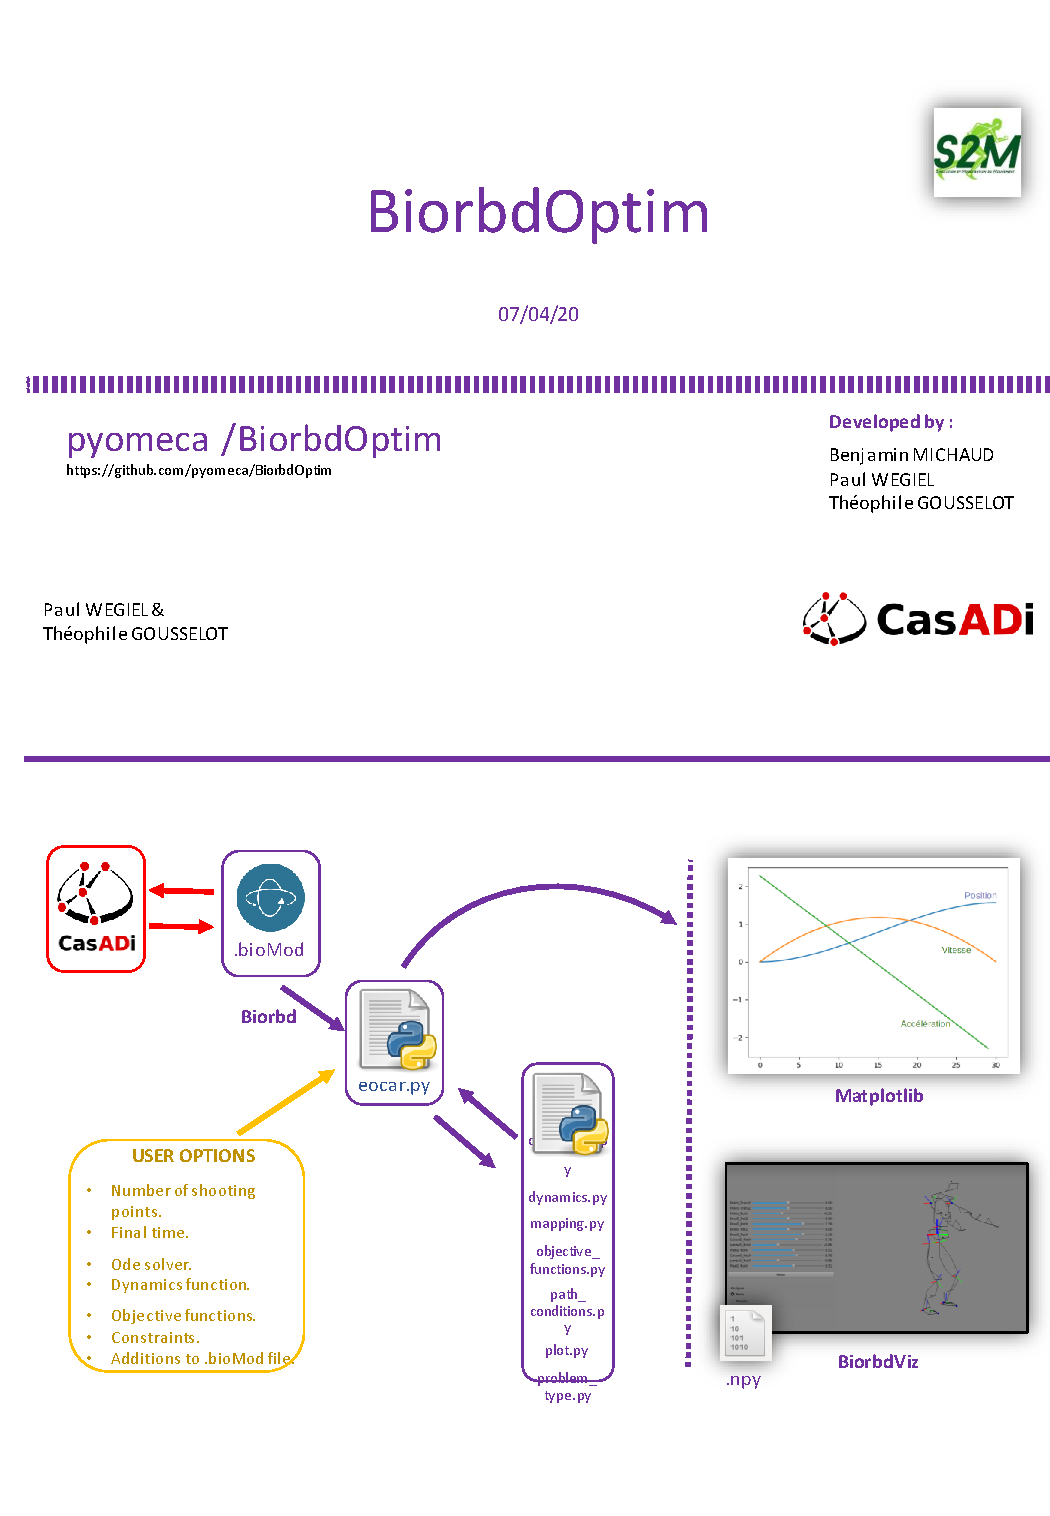
\includepdf[pages=-, width=17cm]{pdf/S2M1.pdf}
\vspace{-0.6cm}
\begin{figure}[h]
\caption{Première présentation à l'attention des membres de l'équipe de commande optimale.}
\end{figure}
\end{center}

\begin{center}
\label{s2m2}
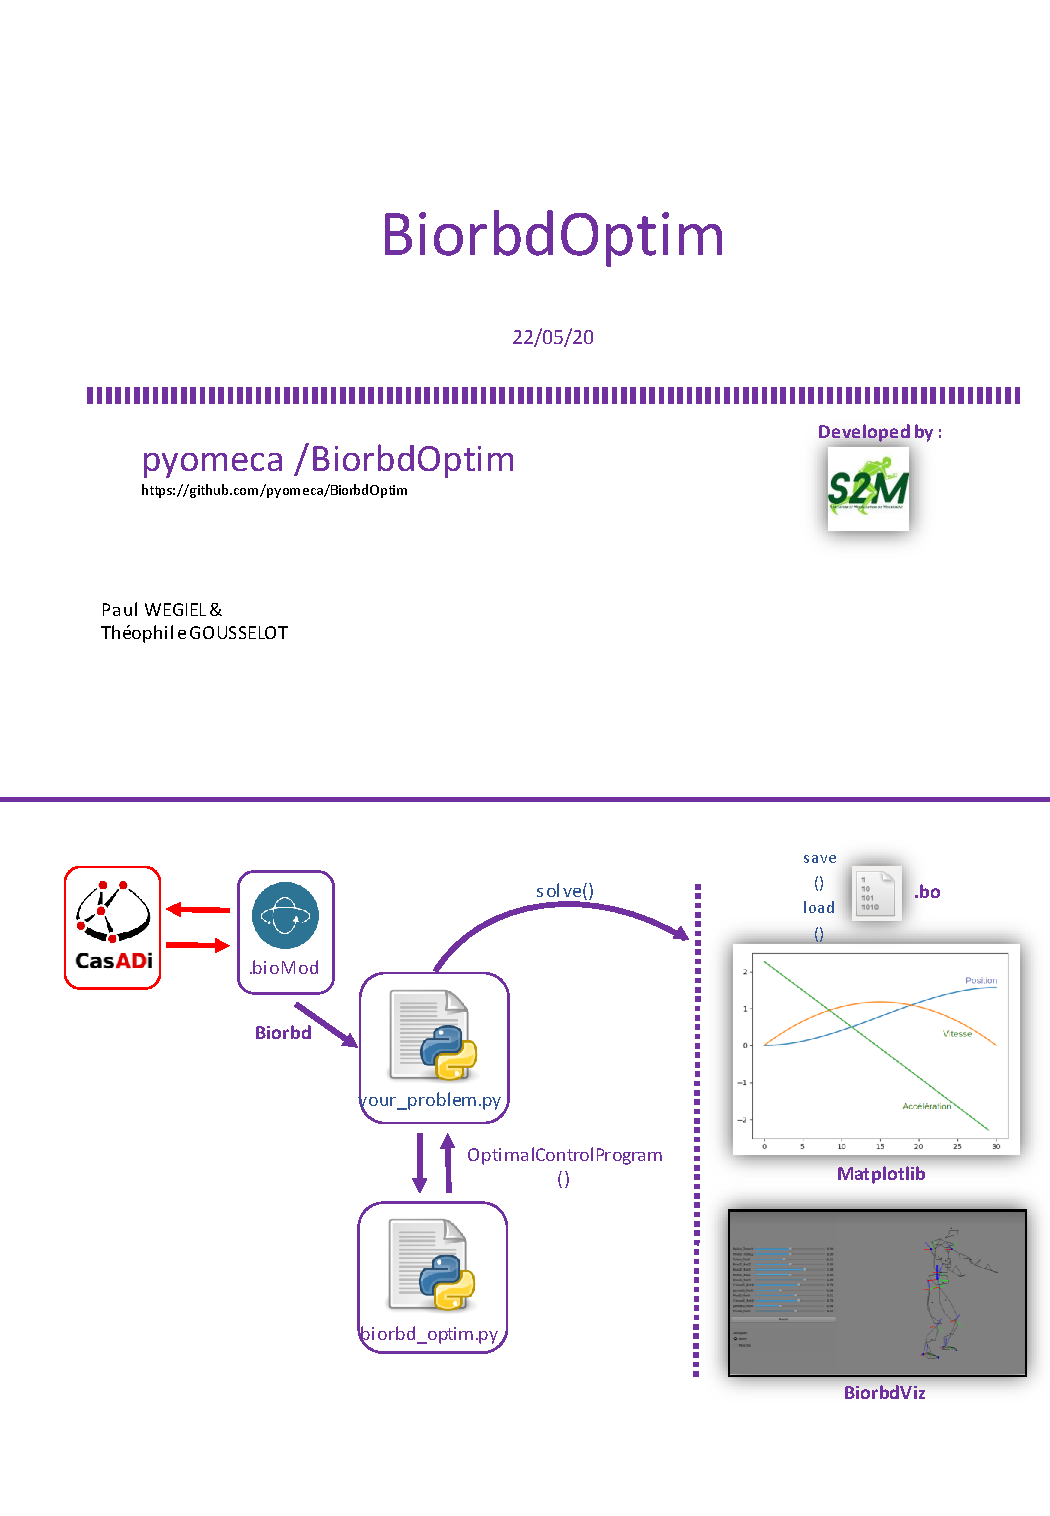
\includepdf[pages=-, width=17cm]{pdf/S2M2.pdf}
\vspace{-0.6cm}
\begin{figure}[h]
\caption{Deuxième présentation à l'attention des membres du laboratoire S2M.}
\end{figure}
\end{center}


\end{appendix}


\backmatter

\bibliographystyle{unsrt} % Le style est mis entre crochets.
\bibliography{rapport_de_stage_gousselot_theophile} % Mon fichier de base de données s'appelle bibli.bib.


Epilogue

\listoffigures
\listoftables


\end{document}


%TODO
% -> ajouter index
% \cite{ref}
% \cite{ref2}

%
% complexité dans les problemes, il ne doit pas y en avoir dans la présentation

%
% Ce n'est pas parcequ'on à beaucoup de temps qu'on peut le perdre !
